\section{Correction résiduelle absolue en \pT\ avec les événements \Gjets}\label{chapter-JERC-section-JES}
L'obtention de la correction résiduelle absolue en \pT\ des jets
ainsi que la correction de leur résolution en énergie
avec les événements \Gjets\ a été un des mes travaux de thèse.
J'ai ainsi traité les données de l'année 2018 et les données \og 2017-UL \fg{} où UL signifie \emph{Ultra-Legacy}.
Il s'agit des données de l'année 2017 qui sont réinterprétées une fois les défauts du détecteurs mieux cernés, par exemple.
\subsection{Jeux de données et sélection des événements}\label{chapter-JERC-section-JES-subsec-evt_select}
\subsubsection{Jeux de données}
%18 data
%     Run2018A-17Sep2018-v2
%     /EGamma/Run2018A-17Sep2018-v2/MINIAOD
%     13654.355526985
%     
%     Run2018B-17Sep2018-v1
%     /EGamma/Run2018B-17Sep2018-v1/MINIAOD
%     7057.825158567
%     
%     Run2018C-17Sep2018-v1
%     /EGamma/Run2018C-17Sep2018-v1/MINIAOD
%     6894.770971269
%     
%     Run2018D-PromptReco-v2
%     /EGamma/Run2018D-PromptReco-v2/MINIAOD
%     31066.589629726
%
%18 MC
%     GJet_Pt-15To6000_RunIIAutumn18MiniAOD-102X
%     /GJet_Pt-15To6000_TuneCP5-Flat_13TeV_pythia8/RunIIAutumn18MiniAOD-102X_upgrade2018_realistic_v15-v1/MINIAODSIM
%     283000.0
%
%17UL data
%     Run2017B-09Aug2019_UL2017-v1
%     /SinglePhoton/Run2017B-09Aug2019_UL2017-v1/MINIAOD
%     4793.961426839
%     
%     Run2017C-09Aug2019_UL2017-v1
%     /SinglePhoton/Run2017C-09Aug2019_UL2017-v1/MINIAOD
%     9631.214820913
%     
%     Run2017D-09Aug2019_UL2017-v1
%     /SinglePhoton/Run2017D-09Aug2019_UL2017-v1/MINIAOD
%     4247.682053046
%     
%     Run2017E-09Aug2019_UL2017-v1
%     /SinglePhoton/Run2017E-09Aug2019_UL2017-v1/MINIAOD
%     9313.642401775
%     
%     Run2017F-09Aug2019_UL2017-v1
%     /SinglePhoton/Run2017F-09Aug2019_UL2017-v1/MINIAOD
%     13539.378417564
%
%
%17UL MC
%     GJets_HT-40To100_RunIISummer19MiniAOD-106X
%     /GJets_HT-40To100_TuneCP5_13TeV-madgraphMLM-pythia8/RunIISummer19UL17MiniAOD-106X_mc2017_realistic_v6-v1/MINIAODSIM
%     18700.0
%     
%     GJets_HT-100To200_RunIISummer19MiniAOD-106X
%     /GJets_HT-100To200_TuneCP5_13TeV-madgraphMLM-pythia8/RunIISummer19UL17MiniAOD-4cores5k_106X_mc2017_realistic_v6-v1/MINIAODSIM
%     8640.0
%     
%     GJets_HT-200To400_RunIISummer19MiniAOD-106X
%     /GJets_HT-200To400_TuneCP5_13TeV-madgraphMLM-pythia8/RunIISummer19UL17MiniAOD-106X_mc2017_realistic_v6-v1/MINIAODSIM
%     2185.0
%     
%     GJets_HT-400To600_RunIISummer19MiniAOD-106X
%     /GJets_HT-400To600_TuneCP5_13TeV-madgraphMLM-pythia8/RunIISummer19UL17MiniAOD-106X_mc2017_realistic_v6-v1/MINIAODSIM
%     259.9
%     
%     GJets_HT-600ToInf_RunIISummer19MiniAOD-106X
%     /GJets_HT-600ToInf_TuneCP5_13TeV-madgraphMLM-pythia8/RunIISummer19UL17MiniAOD-106X_mc2017_realistic_v6-v1/MINIAODSIM
%     85.31 \pm 0.2564
\paragraph{Données réelles}
Les jeux de données réelles utilisés pour 2018 et 2017-UL sont basés sur la présence d'un photon dans l'état final.
Plusieurs périodes sont considérées pour chacune de ces années, celles des collisions \proton\proton, dont la liste et les luminosités correspondantes sont présentés dans les tableaux~\ref{subtab-Runs_and_lumis_2018_GJet} et~\ref{subtab-Runs_and_lumis_2017UL_GJet}.
\begin{table}[h]
\centering
\subcaptionbox{Année 2018.\label{subtab-Runs_and_lumis_2018_GJet}}[.45\textwidth]
{\begin{tabular}{cc}
\toprule
Run & Luminosité (\SI{}{\femto\barn^{-1}})\\
\midrule
A & \num{13.65} \\
B & \num{7.06} \\
C & \num{6.89} \\
D & \num{31.07} \\
\midrule
Total & \num{58.67} \\
\bottomrule
\end{tabular}}
\subcaptionbox{Année 2017-UL.\label{subtab-Runs_and_lumis_2017UL_GJet}}[.45\textwidth]
{\begin{tabular}{cc}
\toprule
Run & Luminosité (\SI{}{\femto\barn^{-1}})\\
\midrule
B & \num{4.79} \\
C & \num{9.63} \\
D & \num{4.25} \\
E & \num{9.31} \\
F & \num{13.54} \\
\midrule
Total & \num{41.52} \\
\bottomrule
\end{tabular}}
\caption{Liste des périodes de prise de données considérées et luminosités correspondantes.}
\label{tab-Runs_and_lumis_2018_and_2017UL_GJet}
\end{table}
\paragraph{Données simulées}
Les simulations utilisées contiennent des événements \Gjets\ de type $\quark\gluon\to\quark\photon$, comme ceux des figures~\ref{subfig-fgraph-gq_qGamma_S} et~\ref{subfig-fgraph-gq_qGamma_T}, et $\quark\quark\to\gluon\photon$, comme celui de la figure~\ref{subfig-fgraph-qq_gGamma}.
Pour l'année 2018, les événements sont générés en un seul jeu de données
à l'aide de \PYTHIA~8~\cite{pythia8.2}
avec les réglages CP5-Flat~\cite{tunes_2019}
et une énergie dans le centre de masse de \SI{13}{\TeV}.
Dans l'état final, un photon d'impulsion transverse comprise entre \num{15} et \SI{6000}{\GeV} est généré.
Pour l'année 2017-UL, les événements sont générés conjointement
à l'aide de \PYTHIA~8~\cite{pythia8.2}
avec les réglages CP5~\cite{tunes_2019}
et
\MADGRAPHc~\cite{madgraph5}
et une énergie dans le centre de masse de \SI{13}{\TeV}.
Dans l'état final, la somme scalaire des impulsions transverses des jets, notée HT, appartient à un intervalle, définissant ainsi cinq jeux de données.
Les sections efficaces des jeux de données d'événements simulés ainsi obtenus sont présentées dans le tableau~\ref{tab-MC_xsec_2018_and_2017UL_GJet}.
\begin{table}[h]
\centering
\begin{tabular}{clc}
\toprule
Année & Caractéristique & Section efficace (\SI{}{\pico\barn})\\
\midrule
2018 & $\pT^{\photon}\in [\num{15}, \num{6000}]\usp\SI{}{\GeV}$ & \num{283000.0}\\
2017-UL & $\text{HT} \in [\num{40}, \num{100}]\usp\SI{}{\GeV}$ & \num{18700.0} \\
2017-UL & $\text{HT} \in [\num{100}, \num{200}]\usp\SI{}{\GeV}$ & \num{8640.0} \\
2017-UL & $\text{HT} \in [\num{200}, \num{400}]\usp\SI{}{\GeV}$ & \num{2185.0} \\
2017-UL & $\text{HT} \in [\num{400}, \num{600}]\usp\SI{}{\GeV}$ & \num{259.9} \\
2017-UL & $\text{HT} > \SI{600}{\GeV}$ & \num{85.31} \\
\bottomrule
\end{tabular}
\caption{Sections efficaces des différents jeux de données \Gjets\ simulés.}
\label{tab-MC_xsec_2018_and_2017UL_GJet}
\end{table}
\subsubsection{Sélection des événements}
Une sélection plus fine des événements à considérer est réalisée lors de l'analyse elle-même.
En effet, les événements souhaités sont ceux contenant un photon avec un ou plusieurs jets;
un des bruits de fond principal provient d'événements multijets où un des jets est identifié à tort comme un photon.
Cette situation peut arriver lorsque ce jet contient de nombreux pions neutres, les \pionnull.
Les \pionnull\ se propagent sur des distances moyennes de \SI{26}{\nano\meter} puis se désintègrent dans \SI{99}{\%} des cas en deux photons~\cite{PDG_booklet_2018}.
Ces particules ne laissent donc aucune trace dans le trajectographe et un dépôt d'énergie dans le ECAL, tout comme un vrai photon issu de l'interaction initiale.
Un tel jet comporte ainsi une signature similaire à un photon d'un événement \Gjet\ autour duquel une activité hadronique existe.
Les topologies de ces deux types d'événements, semblables, sont représentées sur la figure~\ref{fig-Gamma_plus_jet_events_real_faked}.
\begin{figure}[h]
\centering
\subcaptionbox{Topologie d'un événement dijet, dont un jet contient de nombreux \pionnull.\label{subfig-Gamma_plus_jet_basic_event_dijet_faked}}[.45\textwidth]
{\includegraphics[width=.45\textwidth,height=.25\textheight,keepaspectratio]{\PhDthesisdir/tex/Event_displays/JERC/Dijets_pi0s.tex}}
\hfill
\subcaptionbox{Topologie d'un vrai événement \Gjet\ avec un peu d'activité hadronique autour du photon.\label{subfig-Gamma_plus_jet_basic_event_real}}[.45\textwidth]{\includegraphics[width=.45\textwidth,height=.25\textheight,keepaspectratio]{\PhDthesisdir/tex/Event_displays/JERC/Gamma_plus_jet_hadronic_noise.tex}}
\caption{Topologies d'événements \Gjet\ et dijets.}
\label{fig-Gamma_plus_jet_events_real_faked}
\end{figure}
\paragraph{Sélection sur les photons}
Une sélection des photons est appliquée afin de réduire le bruit de fond.
La collaboration CMS propose des critères d'identification des photons (lâche, moyen et strict) s'appuyant sur diverses propriétés du \og candidat \fg{} photon:
\begin{itemize}
\item $H/E$ est le rapport de l'énergie hadronique sur l'énergie électromagnétique associées à l'agglomérat d'énergie du photon.
Un photon est sensé déposer son énergie dans le ECAL et ne laisser aucun signal dans le HCAL.
Une faible valeur de $H/E$ est donc compatible avec un photon.
\item $\sigma_{i\eta i\eta}$ est l'étalement en $\eta$ du dépôt d'énergie dans le ECAL.
Cette observable est reliée à la forme de la gerbe électromagnétique, moins étalée pour un photon que pour un électron.
Une faible valeur de $\sigma_{i\eta i\eta}$ est donc compatible avec un photon.
\item $I_{CH}$ est l'isolation vis-à-vis des hadrons chargés.
Elle se définit comme le ratio entre la somme des impulsions transverses de tous les hadrons chargés situés à une distance $\Delta R$ du candidat photon dans le plan $(\eta,\phi)$ inférieure à \num{0.3} et l'impulsion transverse du candidat photon lui-même.
\item $I_{NH}$ est l'isolation vis-à-vis des hadrons neutres, analogue à $I_{CH}$.
\item $I_{\photon}$ est l'isolation vis-à-vis des photons autres que le candidat lui-même, analogue à $I_{CH}$.
\end{itemize}
À cet ensemble de variables dont une valeur maximale est admise pour l'identification des photons s'ajoute $R_9$, définie comme
\begin{equation}
R_9 = \frac{E_{3\times3}}{E_{SC}}
\label{eq-R9_definition}
\end{equation}
avec
$E_{3\times3}$ la somme des énergies dans les cristaux du ECAL formant un carré de trois cristaux de côté centré sur le cristal contenant le plus d'énergie dans le \emph{supercluster}\footnote{Le \emph{supercluster} est défini dans la section~\ifref{chapter-LHC-section-evt_reco-subsec-ptc_ID}{\ref{chapter-LHC-section-evt_reco-subsec-ptc_ID}}{4.2} du chapitre\ifref{chapter-LHC}{~\ref{chapter-LHC}}{ \og Dispositif expérimental \fg}.}
et
$E_{SC}$
l'énergie dans le \emph{supercluster}~\cite{photon_ID_2015}.
Dans l'analyse des événements \Gjets, il est requis que $R_9 > \num{0.90}$.
\par Les variables d'isolation sont corrigées afin de prendre en compte l'empilement, on considère alors $I^\text{corr}$ au lieu de $I$, telle que
\begin{equation}
I^\text{corr} = \max\left( I - \rho \times \mathcal{E_A} , 0\right)
\end{equation}
où $\mathcal{E_A}$ est l'aire effective, \ie\ la fraction de l'espace $(\eta,\phi)$ correspondant à la zone d'isolation à corriger pour l'empilement. Les valeurs des aires effectives utilisées sont présentées dans le tableau~\ref{tab-CutBasedPhotonIdentificationRun2-effective_areas}.
Les coupures définissant les différents critères d'identification des photons ainsi que leurs efficacités d'identification et de réjection sont résumées dans le tableau~\ref{tab-CutBasedPhotonIdentificationRun2}.
\begin{table}[h]
\centering
\begin{tabular}{cccc}
\toprule
Région & Hadrons chargés & Hadrons neutres & Photons \\
\midrule
$\abs{\eta} \leq \num{1.0}$ & \num{0.0112} & \num{0.0668} & \num{0.1113} \\
$\num{1.0} < \abs{\eta} \leq \num{1.479}$ & \num{0.0108} & \num{0.1054} & \num{0.0953} \\
$\num{1.479} < \abs{\eta} \leq \num{2.0}$ & \num{0.0106} & \num{0.0786} & \num{0.0619} \\
$\num{2.0} < \abs{\eta} \leq \num{2.2}$ & \num{0.01002} & \num{0.0233} & \num{0.0837} \\
$\num{2.2} < \abs{\eta} \leq \num{2.3}$ & \num{0.0098} & \num{0.0078} & \num{0.1070} \\
$\num{2.3} < \abs{\eta} \leq \num{2.4}$ & \num{0.0089} & \num{0.0028} & \num{0.1212} \\
$\abs{\eta} > \num{2.4}$ & \num{0.0087} & \num{0.0137} & \num{0.1466} \\
\bottomrule
\end{tabular}
\caption[Aires effectives de correction de l'isolation du photon.]{Valeurs de l'aire effective $\mathcal{E_A}$ utilisée pour corriger la contribution de l'empilement aux isolations des photons vis-à-vis des autres particules.}
\label{tab-CutBasedPhotonIdentificationRun2-effective_areas}
\end{table}
\begin{table}[h]
\centering\small
\begin{tabularx}{\textwidth}{Xcccccc}
\toprule
Critère & \multicolumn{2}{c}{Lâche} & \multicolumn{2}{c}{Moyen} & \multicolumn{2}{c}{Strict} \\
\cmidrule(lr){2-3}\cmidrule(lr){4-5}\cmidrule(lr){6-7}
Région & Barillet & Bouchon & Barillet & Bouchon & Barillet & Bouchon\\
\midrule
Efficacité & \SI{90.08}{\%} & \SI{90.65}{\%} & \SI{80.29}{\%} & \SI{80.08}{\%} & \SI{70.24}{\%} & \SI{70.13}{\%} \\
Réjection & \SI{86.25}{\%} & \SI{76.72}{\%} & \SI{89.36}{\%} & \SI{81.85}{\%} & \SI{90.97}{\%} & \SI{84.55}{\%} \\
\midrule
$H/E$ & \num{0.04596} & \num{0.0590} & \num{0.02197} & \num{0.0326} & \num{0.02148} & \num{0.0321} \\
$\sigma_{i\eta i\eta}$ & \num{0.0106} & \num{0.0272} & \num{0.01015} & \num{0.0272} & \num{0.00996} & \num{0.0271} \\
$I_{CH}^\text{corr}$ & \num{1.694} & \num{2.089} & \num{1.141} & \num{1.051} & \num{0.65} & \num{0.517} \\
\multirow{3}{*}{$I_{NH}^\text{corr} \!\!\!\hphantom{I_{\photon}^\text{corr}} \left\lbrace \begin{matrix} \vphantom{0} \\ \vphantom{0} \\ \vphantom{0} \end{matrix} \right. $} & $\num{24.032}$& $\num{19.722}$& $\num{1.189}$& $\num{2.718}$& $\num{0.317}$& $\num{2.716}$\\
& $+ \num{0.01512} \, \pT$& $+ \num{0.011} \, \pT$& $+ \num{0.01512} \, \pT$& $+ \num{0.0117} \, \pT$& $+ \num{0.01512} \, \pT$& $+ \num{0.0117} \, \pT$ \\
& $+ \num{2.259} \pT^{\!2} \! / 10^5$ & $+ \num{2.3} \pT^{\!2} \! / 10^5$ & $+ \num{2.259} \pT^{\!2} \! / 10^5$ & $+ \num{2.3} \pT^{\!2} \! / 10^5$ & $+ \num{2.259} \pT^{\!2} \! / 10^5$ & $+ \num{2.3} \pT^{\!2} \! / 10^5$ \\
\multirow{2}{*}{$I_{\photon}^\text{corr} \!\!\!\hphantom{I_{NH}^\text{corr}} \left\lbrace \begin{matrix} \vphantom{0} \\ \vphantom{0} \end{matrix} \right. $} & $\num{2.876}$ & $\num{4.162}$ & $\num{2.08}$ & $\num{3.867}$ & $\num{2.044}$ & $\num{3.032}$ \\
& $+ \num{0.004017} \, \pT$ & $+ \num{0.0037} \, \pT$ & $+ \num{0.004017} \, \pT$ & $+ \num{0.0037} \, \pT$ & $+ \num{0.004017} \, \pT$ & $+ \num{0.0037} \, \pT$ \\
\bottomrule
\end{tabularx}
\caption[Coupures utilisées pour l'identification des photons.]{Valeurs maximales des observables considérées pour l'identification des photons selon le critère utilisé et la région du détecteur dans laquelle se trouve le candidat photon (barillet pour $\abs{eta} < \num{1.479}$, bouchon sinon).}
\label{tab-CutBasedPhotonIdentificationRun2}
\end{table}
\par Le critère d'identification des photons retenu dans l'analyse est le critère strict.
Seuls les photons situés dans le barillet sont utilisés car ils présentent la meilleure résolution.
La figure~\ref{fig-chapter-JERC-section-pheno-GJets-photon_resolution}, page~\pageref{fig-chapter-JERC-section-pheno-GJets-photon_resolution}, montre en effet que ces photons possède une résolution relative en énergie de l'ordre de \SI{1}{\%}, contre environ \SI{2.5}{\%} pour les photons des bouchons.
Une coupure sur leur pseudo-rapidité est donc appliquée, telle que $\abs{\eta} < \num{1.305}$.
\par \todo{Barrel photon study if done in service task, else small paragraph on this idea}
\paragraph{Sélection sur les jets}
Les événements présentant un unique photon sélectionné d'après les critères précédents sont retenus.
Avec ce photon doit être présent au moins un jet reconstruit à l'aide de l'algorithme anti-\kT~\cite{Cacciari_antikT} avec un paramètre $R=\num{0.4}$ et respectant les critères définis dans le tableau~\ref{tab-chapter-JERC-section-jets_reco-subsec-jetID-2018} pour les données de 2018 et ceux du tableau~\ref{tab-chapter-JERC-section-jets_reco-subsec-jetID-2017UL} pour les données de 2017-UL.
Ces critères permettent de rejeter les jets issus du bruit de fond avec une efficacité de \SI{99}{\%}.
\par Les jets ainsi sélectionnés sont calibrés en énergie en suivant la procédure décrite dans la section~\ref{chapter-JERC-section-CMS} jusqu'à la correction résiduelle relative en $\eta$ incluse. Ils sont alors triés par impulsion transverse décroissante.
Pour s'assurer d'une bonne balance dans le plan transverse entre le photon et le premier jet, \ie\ celui d'impulsion transverse la plus grande, seuls les événements proposant un écart angulaire entre le photon et le jet supérieur à \SI{2.8}{\rad} sont considérés dans la suite.
Le photon et le jet sont donc dos à dos dans le plan transverse, ce qui correspond à la situation illustrée figures~\ref{subfig-Gamma_plus_jet_basic_event}, \ref{subfig-Gamma_plus_two_jets} et~\ref{subfig-Gamma_plus_jet_basic_event_real}.
\par Si un second jet d'impulsion transverse supérieure à \SI{10}{\GeV} est présent, l'événement est rejeté si $\alpha>\num{0.3}$ où $\alpha$ est défini dans l'équation~\eqref{eq-chapter-JERC-definition_alpha}, page~\pageref{eq-chapter-JERC-definition_alpha}.
L'événement est également rejeté si un lepton (électron ou muon) isolé, en pratique hors des jets, est présent.
\par \todo{graph pureté?}
\paragraph{Sélection sur le chemin de déclenchement}
Dans le cas des données réelles, l'événement est sauvegardé si un chemin de déclenchement est activé\footnote{Le chemin de déclenchement est abordé dans la section~\ifref{chapter-LHC-section-CMS-subsec-data_taking}{\ref{chapter-LHC-section-CMS-subsec-data_taking}}{2.7} du chapitre\ifref{chapter-LHC}{~\ref{chapter-LHC}}{ \og Dispositif expérimental \fg}.}.
Seuls les événements dont le photon retenu correspond au photon du chemin de déclenchement sont retenus.
Il existe plusieurs chemins de déclenchement en fonction de l'impulsion du photon.
Certains de ces chemins proposent une quantité trop importante d'événements à sauvegarder et pourraient saturer la chaîne d'acquisition.
Pour éviter cette saturation, seule une fraction des événements passant un tel chemin de déclenchement sont effectivement sauvegardés.
Cette fraction est nommée \emph{prescale}.
Chaque chemin de déclenchement possède ainsi son \emph{prescale}.
Afin de ne pas introduire de biais dû à ces \emph{prescales} dans l'analyse, un intervalle d'impulsion transverse du photon retenu est défini pour chaque chemin de déclenchement utilisé.
Il est ainsi requis que le photon retenu soit le photon du chemin de déclenchement correspondant à l'intervalle dans lequel se trouve son impulsion transverse.
Les différents chemins de déclenchement, leurs \emph{prescales} et intervalles d'impulsion transverse sont présentés dans le tableau~\ref{tab-HLT_pT_precales_18_and_17UL}.
\begin{table}
\centering
\begin{tabular}{lccc}
\toprule
Chemin de déclenchement & $\pT^{\photon}$ (\SI{}{\GeV}) & \emph{Prescale} 2018 & \emph{Prescale} 2017-UL\\
\midrule
%\inlinepython{HLT_Photon33} & $[\num{40}, \num{60}[$ & \num{4.0115375867e-5} & \num{3.434860938821936e-4} \\
%\inlinepython{HLT_Photon50_R9Id90_HE10_IsoM} & $[\num{60}, \num{85}[$ & \num{3.9473720141e-3} & \num{7.40465688874224e-3} \\
%\inlinepython{HLT_Photon75_R9Id90_HE10_IsoM} & $[\num{85}, \num{105}[$ & \num{0.0156656382257} & \num{0.03195516364518142} \\
%\inlinepython{HLT_Photon90_R9Id90_HE10_IsoM} & $[\num{105}, \num{130}[$ & \num{0.0312899931745} & \num{0.0636323095006467} \\
%\inlinepython{HLT_Photon120_R9Id90_HE10_IsoM} & $[\num{130}, \num{175}[$ & \num{0.125036122867} & \num{0.18787162142132302} \\
%\inlinepython{HLT_Photon165_R9Id90_HE10_IsoM} & $[\num{175}, \num{230}[$ & \num{0.250030962458} & \num{0.6823580953102895} \\
%\inlinepython{HLT_Photon200} & $[\num{230}, +\infty$ & \num{1} & \num{1} \\
\inlinepython{HLT_Photon33} & $[\num{40}, \num{60}[$ & \num{4.01154e-5} & \num{3.43486e-4} \\
\inlinepython{HLT_Photon50_R9Id90_HE10_IsoM} & $[\num{60}, \num{85}[$ & \num{3.94737e-3} & \num{7.40466e-3} \\
\inlinepython{HLT_Photon75_R9Id90_HE10_IsoM} & $[\num{85}, \num{105}[$ & \num{0.0156656} & \num{0.0319552} \\
\inlinepython{HLT_Photon90_R9Id90_HE10_IsoM} & $[\num{105}, \num{130}[$ & \num{0.0312900} & \num{0.0636323} \\
\inlinepython{HLT_Photon120_R9Id90_HE10_IsoM} & $[\num{130}, \num{175}[$ & \num{0.125036} & \num{0.187872} \\
\inlinepython{HLT_Photon165_R9Id90_HE10_IsoM} & $[\num{175}, \num{230}[$ & \num{0.250031} & \num{0.682358} \\
\inlinepython{HLT_Photon200} & $[\num{230}, +\infty [$ & \num{1} & \num{1} \\
\bottomrule
\end{tabular}
\caption[Chemins de déclenchement.]{Chemins de déclenchement, intervalles d'impulsion transverse du photon et \emph{prescales} utilisés.}
\label{tab-HLT_pT_precales_18_and_17UL}
\end{table}
\par Par exemple, un photon d'impulsion transverse \SI{95}{\GeV} doit avoir déclenché le chemin nommé \inlinepython{HLT_Photon75_R9Id90_HE10_IsoM}.
Ce chemin de déclenchement requière un photon d'impulsion transverse minimale \SI{75}{\GeV}.
Ce même photon déclenche donc potentiellement le chemin nommé \inlinepython{HLT_Photon90_R9Id90_HE10_IsoM}.
Utiliser un écart minimal entre l'impulsion du photon et l'impulsion minimale requise au déclenchement du chemin permet de se placer au plateau d'efficacité maximale du chemin de déclenchement.
Des biais dus à la calibration du photon sont également évités grâce à cette méthode.
\subsection{Analyse}\label{chapter-JERC-section-JES-subsec-analyse}
\paragraph{Intervalles de $\pT^{\photon}$}
L'analyse a pour but de déterminer la correction résiduelle absolue en \pT\ des jets, définie dans la section~\ref{chapter-JERC-section-CMS-subsec-residuals}.
Pour cela, l'écart à l'unité du rapport moyen des réponses des jets dans les données réelles et simulées est déterminé dans différents intervalles de $\pT^{\photon}$, listé dans le tableau~\ref{tab-pT_photon_intervalles}.
Ces intervalles sont une subdivision des intervalles définis pour les chemin de déclenchement dans le tableau~\ref{tab-HLT_pT_precales_18_and_17UL}.
\begin{table}[h]
\centering
\begin{tabular}{cccc}
\toprule
$[\num{40}, \num{50}[$ & $[\num{50}, \num{60}[$ & $[\num{60}, \num{85}[$ & $[\num{85}, \num{105}[$ \\
$[\num{105}, \num{130}[$ & $[\num{130}, \num{175}[$ & $[\num{175}, \num{230}[$ & $[\num{230}, \num{300}[$ \\
$[\num{300}, \num{400}[$ & $[\num{400}, \num{500}[$ & $[\num{500}, \num{700}[$ & $[\num{700}, \num{1000}[$ \\
$[\num{1000}, \num{3000}]$ \\
\bottomrule
\end{tabular}
\caption[Intervalles de $\pT^{\photon}$.]{Intervalles de $\pT^{\photon}$ en \SI{}{\GeV}.}
\label{tab-pT_photon_intervalles}
\end{table}
\paragraph{Intervalles de $\abs{\eta^\text{jet}}$}
La calibration en énergie des jets dépend fortement de la région du détecteur dans lequel le jet laisse un signal, comme le montre la figure~\ref{fig-simulated_jet_response_RunII} en page~\pageref{fig-simulated_jet_response_RunII}.
Cet effet est dû aux différentes technologies utilisées ainsi qu'au vieillissement non uniforme du détecteur.
Des intervalles de pseudo-rapidité du jet sont ainsi définis dans les tableaux~\ref{tab-eta_jet_intervalles_large} et~\ref{tab-eta_jet_intervalles_fin} afin de séparer le traitement de ces différentes régions.
Des intervalles larges sont utilisés pour~\todo{?}, et des plus fins pour~\todo{?}.
\begin{table}[h]
\centering
\begin{tabular}{cccc}
\toprule
$[\num{0}, \num{0.783}[$ & $[\num{0.783}, \num{1.305}[$ & $[\num{1.305}, \num{1.93}[$ & $[\num{1.93}, \num{2.5}[$ \\
$[\num{2.5}, \num{2.964}[$ & $[\num{2.964}, \num{3.2}[$ & $[\num{3.2}, \num{5.191}[$ &  \\
\bottomrule
\end{tabular}
\caption{Intervalles larges de $\abs{\eta^\text{jet}}$.}
\label{tab-eta_jet_intervalles_large}
\end{table}
\begin{table}[h]
\centering
\begin{tabular}{cccccc}
\toprule
$[\num{0}, \num{0.261}[$ & $[\num{0.261}, \num{0.522}[$ & $[\num{0.522}, \num{0.783}[$ & $[\num{0.783}, \num{1.044}[$ & $[\num{1.044}, \num{1.305}[$ & $[\num{1.305}, \num{1.479}[$ \\
$[\num{1.479}, \num{1.653}[$ & $[\num{1.653}, \num{1.930}[$ & $[\num{1.930}, \num{2.172}[$ & $[\num{2.172}, \num{2.322}[$ & $[\num{2.322}, \num{2.500}[$ & $[\num{2.500}, \num{2.650}[$ \\
$[\num{2.650}, \num{2.853}[$ & $[\num{2.853}, \num{2.964}[$ & $[\num{2.964}, \num{3.319}[$ & $[\num{3.319}, \num{3.489}[$ & $[\num{3.489}, \num{3.839}[$ & $[\num{3.839}, \num{5.191}[$ \\
\bottomrule
\end{tabular}
\caption{Intervalles fins de $\abs{\eta^\text{jet}}$.}
\label{tab-eta_jet_intervalles_fin}
\end{table}
\paragraph{Pondération par l'empilement}
Le profil d'empilement, \ie\ la densité de probabilité du nombre d'interactions d'empilement, dépend de la période de la prise de données et du chemin de déclenchement par lequel l'événement est retenu. Ces dépendances sont illustrées sur les graphiques des figures~\ref{fig-PU_profile_18} et~\ref{fig-PU_profile_17UL}.
Les événements simulés sont ainsi pondérés afin que leur distribution du nombre d'interactions d'empilement soit similaire à celle dans les données réelles, en prenant en compte la double dépendance avec la période de prise de donnée et le chemin de déclenchement.
\begin{figure}[p]
\centering
\subcaptionbox{Run 2018 A.\label{subfig-PU_profile_18_A}}[.45\textwidth]
{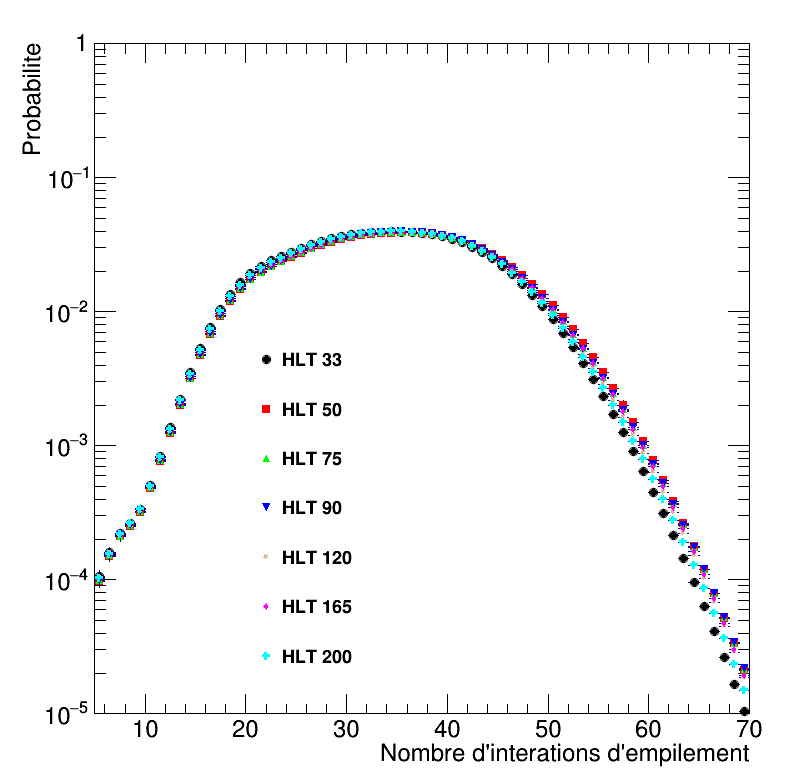
\includegraphics[width=.45\textwidth]{\PhDthesisdir/contents/chapter-JERC/JES/my_plots/PUreweighting/2018/with_header/PU_HLT_profiles_run2018A_only_L2Res.tex}}
\hfill
\subcaptionbox{Run 2018 B.\label{subfig-PU_profile_18_B}}[.45\textwidth]
{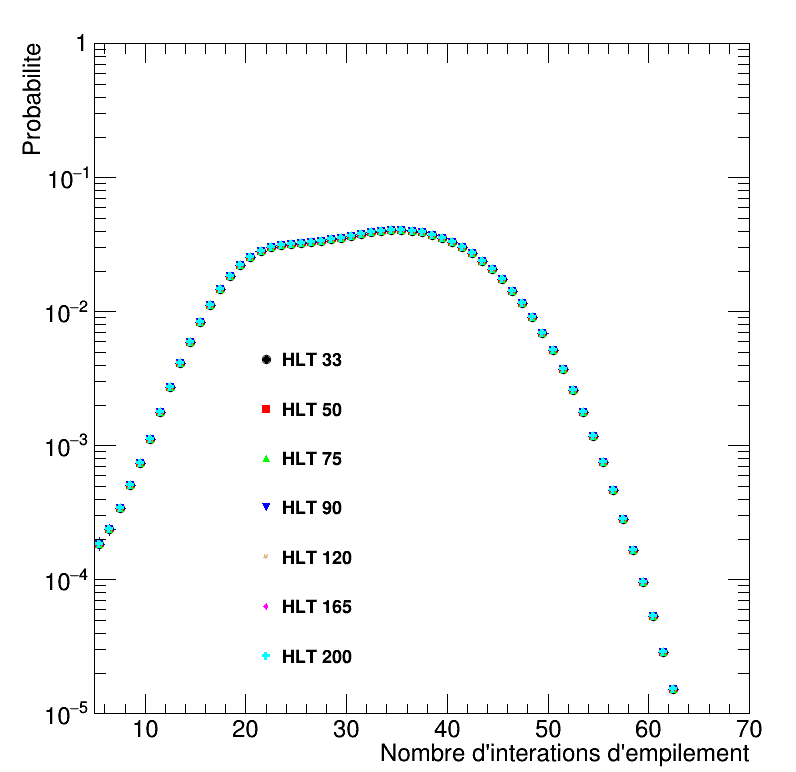
\includegraphics[width=.45\textwidth]{\PhDthesisdir/contents/chapter-JERC/JES/my_plots/PUreweighting/2018/with_header/PU_HLT_profiles_run2018B_only_L2Res.tex}}

\vfill

\subcaptionbox{Run 2018 C.\label{subfig-PU_profile_18_C}}[.45\textwidth]
{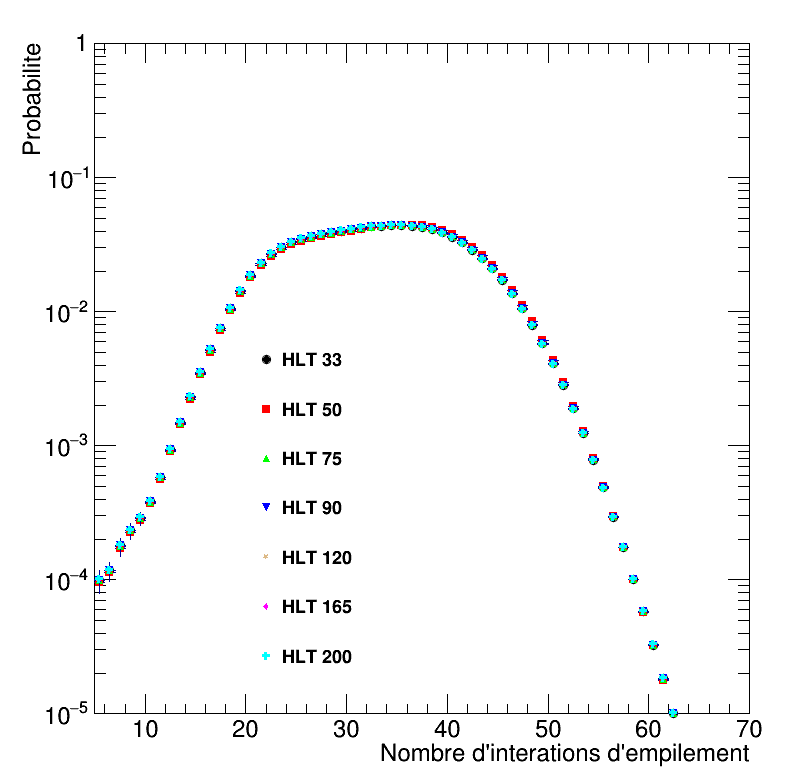
\includegraphics[width=.45\textwidth]{\PhDthesisdir/contents/chapter-JERC/JES/my_plots/PUreweighting/2018/with_header/PU_HLT_profiles_run2018C_only_L2Res.tex}}
\hfill
\subcaptionbox{Run 2018 D.\label{subfig-PU_profile_18_D}}[.45\textwidth]
{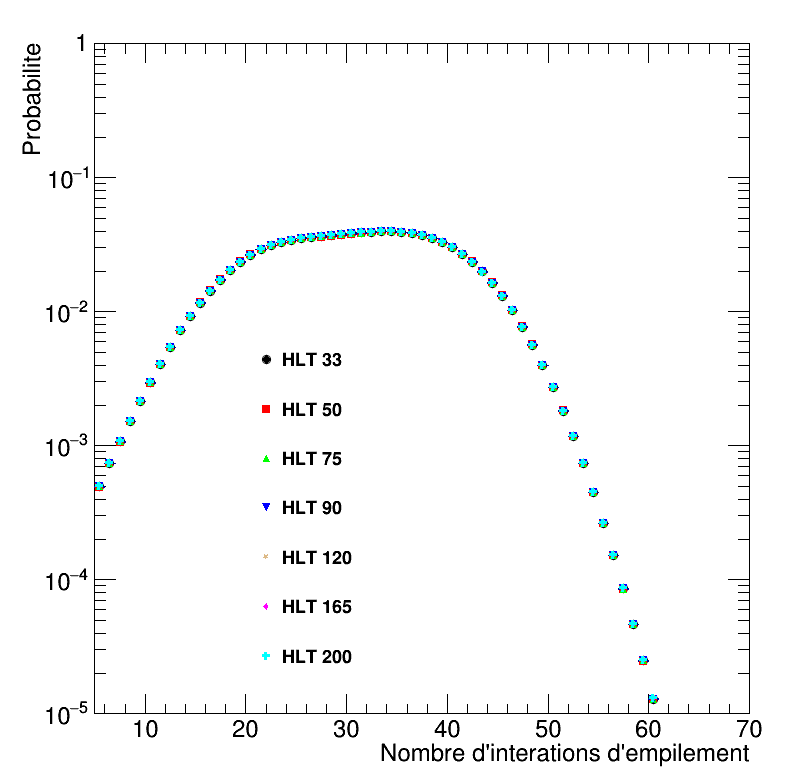
\includegraphics[width=.45\textwidth]{\PhDthesisdir/contents/chapter-JERC/JES/my_plots/PUreweighting/2018/with_header/PU_HLT_profiles_run2018D_only_L2Res.tex}}

\vfill

\subcaptionbox{Run 2018 ABC.\label{subfig-PU_profile_18_ABC}}[.45\textwidth]
{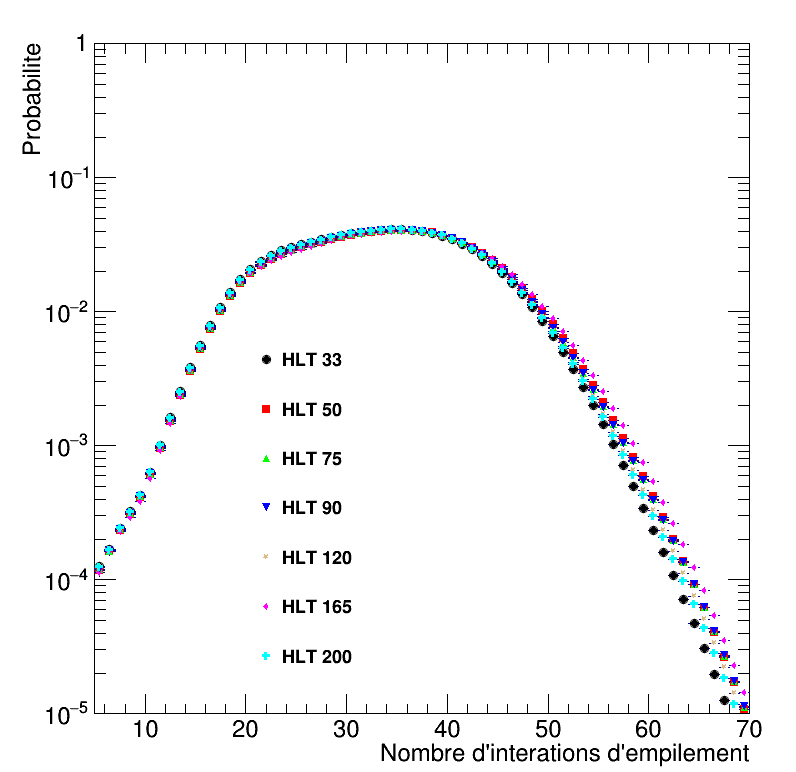
\includegraphics[width=.45\textwidth]{\PhDthesisdir/contents/chapter-JERC/JES/my_plots/PUreweighting/2018/with_header/PU_HLT_profiles_run2018ABC_only_L2Res.tex}}
\hfill
\subcaptionbox{Run 2018 ABCD.\label{subfig-PU_profile_18_ABCD}}[.45\textwidth]
{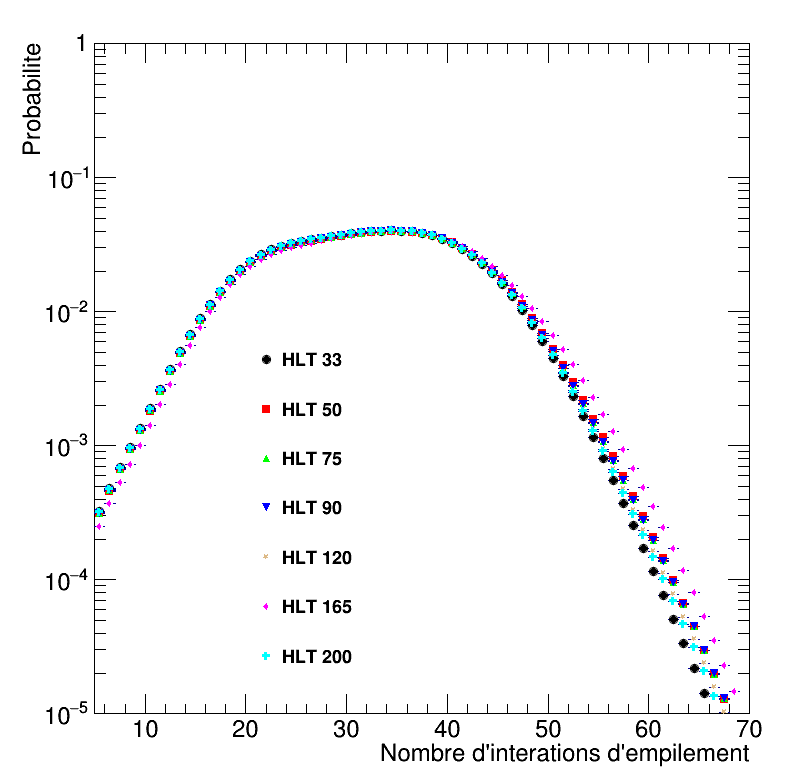
\includegraphics[width=.45\textwidth]{\PhDthesisdir/contents/chapter-JERC/JES/my_plots/PUreweighting/2018/with_header/PU_HLT_profiles_run2018ABCD_only_L2Res.tex}}

\caption{Densités de probabilité du nombre d'interactions d'empilement $N_\text{PU}$ pour les périodes de prises de données de 2018.}
\label{fig-PU_profile_18}
\end{figure}
\begin{figure}[p]
\centering
\subcaptionbox{Run 2017-UL B.\label{subfig-PU_profile_17UL_B}}[.45\textwidth]
{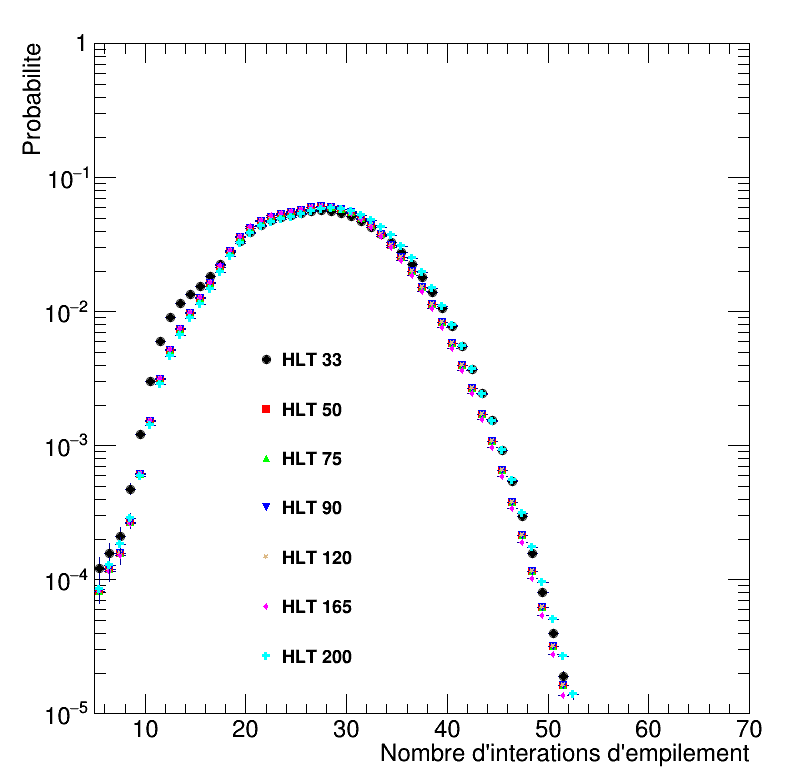
\includegraphics[width=.45\textwidth]{\PhDthesisdir/contents/chapter-JERC/JES/my_plots/PUreweighting/2017UL/with_header/PU_HLT_profiles_run2017B_only_L2Res.tex}}
\hfill
\subcaptionbox{Run 2017-UL C.\label{subfig-PU_profile_17UL_C}}[.45\textwidth]
{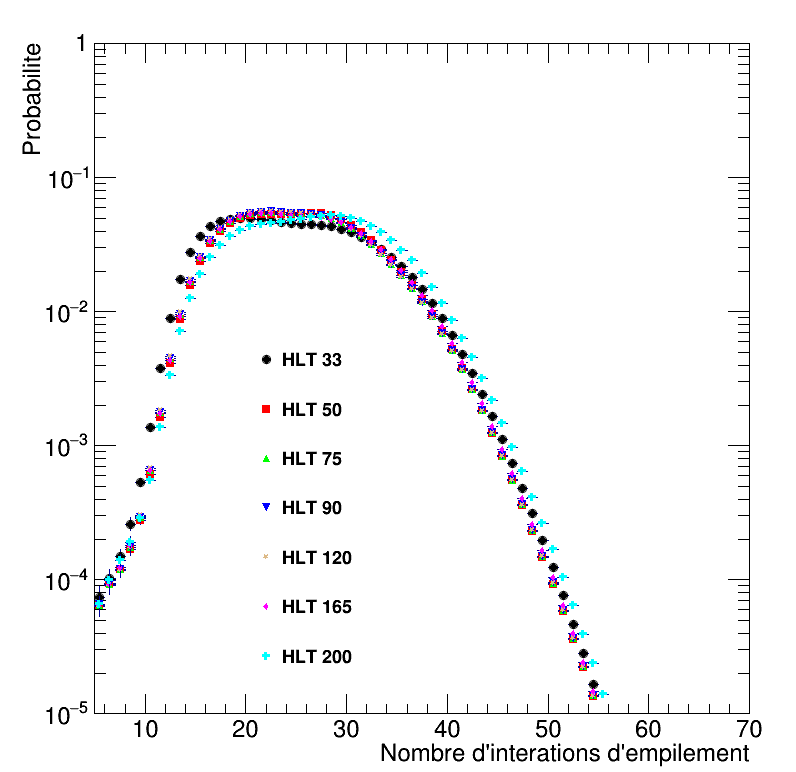
\includegraphics[width=.45\textwidth]{\PhDthesisdir/contents/chapter-JERC/JES/my_plots/PUreweighting/2017UL/with_header/PU_HLT_profiles_run2017C_only_L2Res.tex}}

\vfill

\subcaptionbox{Run 2017-UL D.\label{subfig-PU_profile_17UL_D}}[.45\textwidth]
{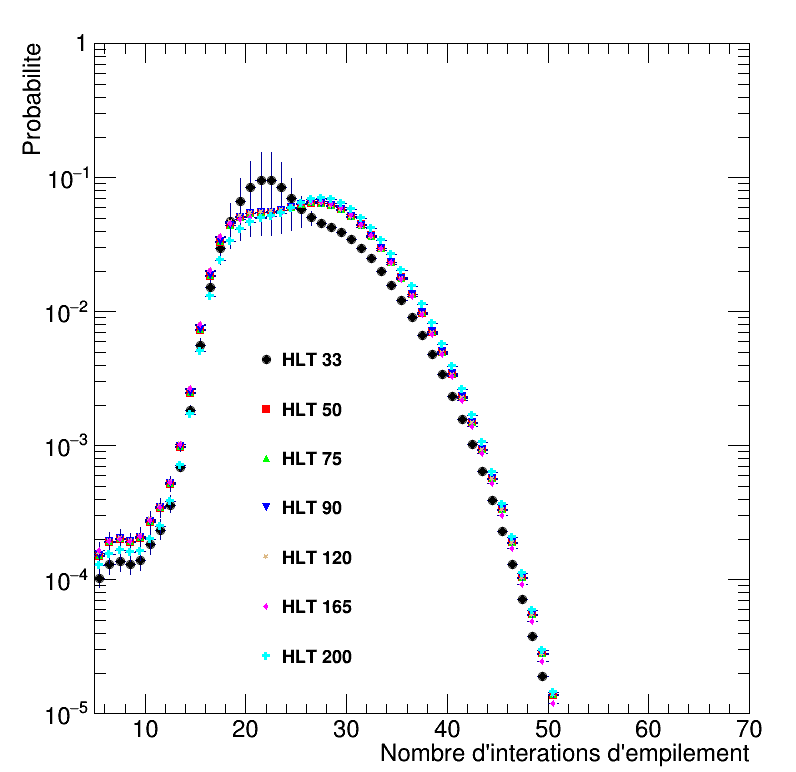
\includegraphics[width=.45\textwidth]{\PhDthesisdir/contents/chapter-JERC/JES/my_plots/PUreweighting/2017UL/with_header/PU_HLT_profiles_run2017D_only_L2Res.tex}}
\hfill
\subcaptionbox{Run 2017-UL E.\label{subfig-PU_profile_17UL_E}}[.45\textwidth]
{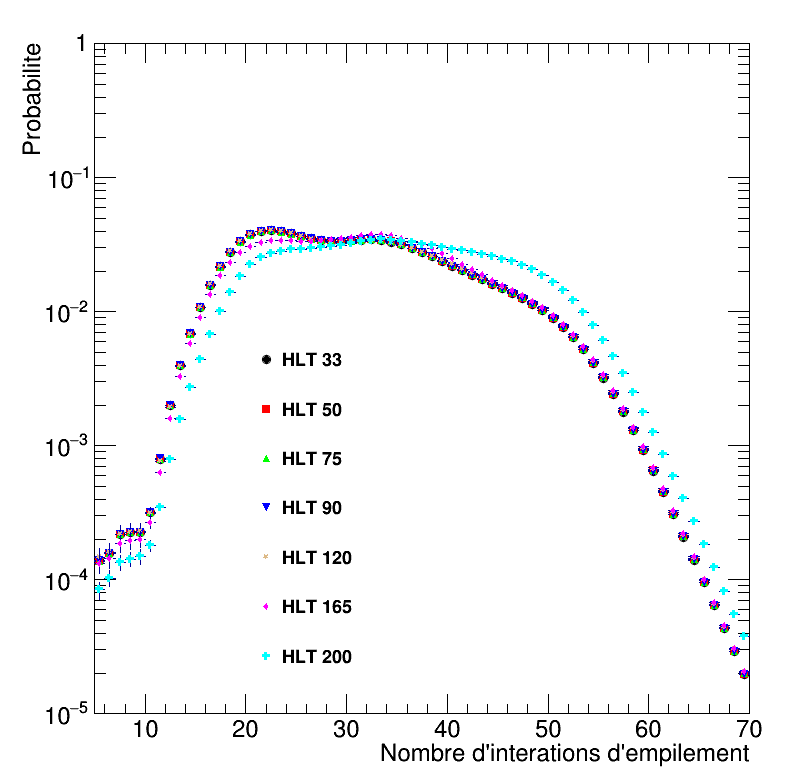
\includegraphics[width=.45\textwidth]{\PhDthesisdir/contents/chapter-JERC/JES/my_plots/PUreweighting/2017UL/with_header/PU_HLT_profiles_run2017E_only_L2Res.tex}}

\vfill

\subcaptionbox{Run 2017-UL F.\label{subfig-PU_profile_17UL_F}}[.45\textwidth]
{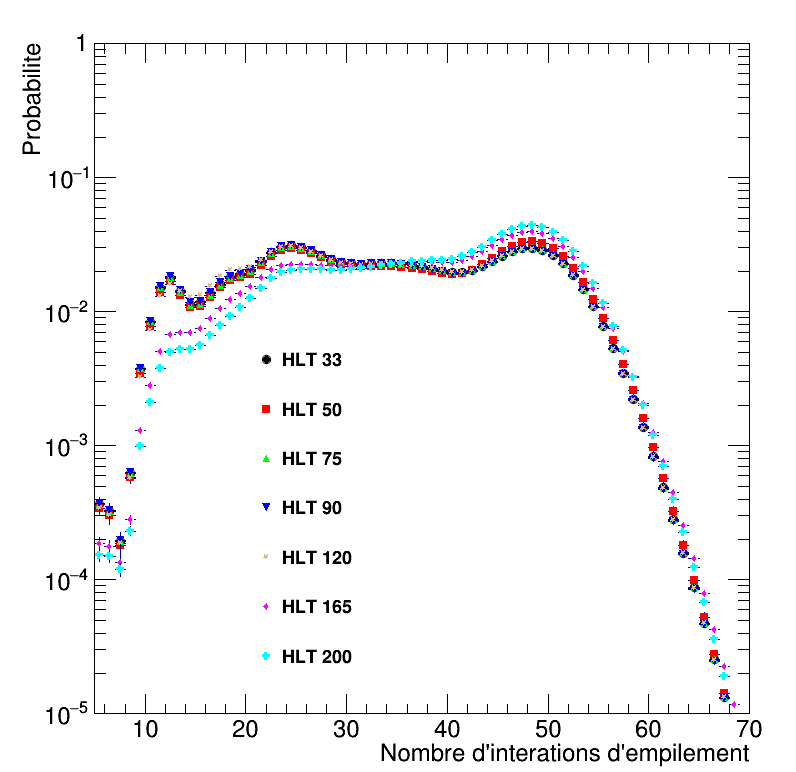
\includegraphics[width=.45\textwidth]{\PhDthesisdir/contents/chapter-JERC/JES/my_plots/PUreweighting/2017UL/with_header/PU_HLT_profiles_run2017F_only_L2Res.tex}}
\hfill
\subcaptionbox{Run 2017-UL BCDEF.\label{subfig-PU_profile_17UL_BCDEF}}[.45\textwidth]
{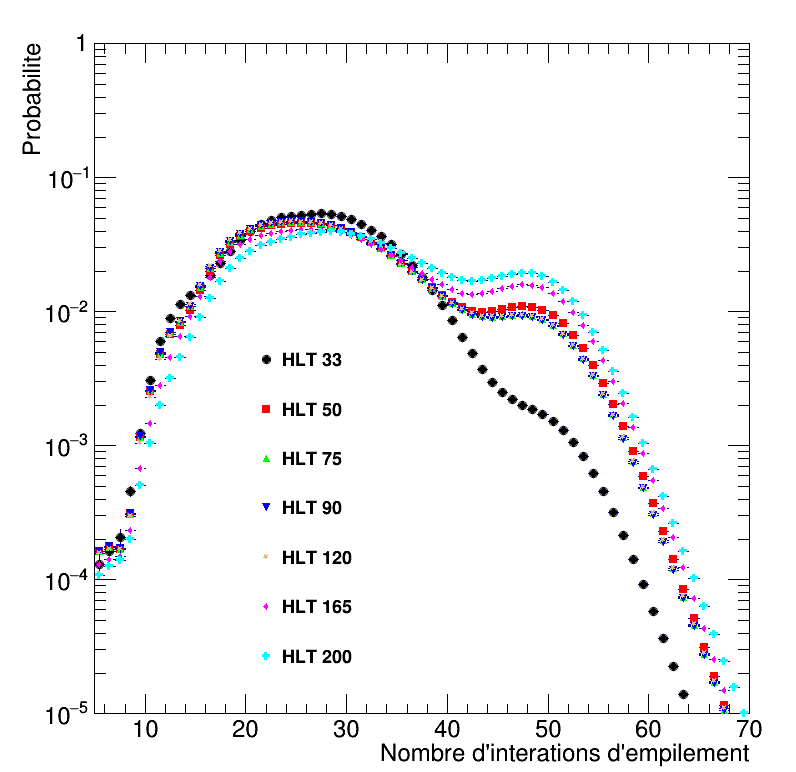
\includegraphics[width=.45\textwidth]{\PhDthesisdir/contents/chapter-JERC/JES/my_plots/PUreweighting/2017UL/with_header/PU_HLT_profiles_run2017BCDEF_only_L2Res.tex}}

\caption{Densités de probabilité du nombre d'interactions d'empilement $N_\text{PU}$ pour les périodes de prises de données de 2017-UL.}
\label{fig-PU_profile_17UL}
\end{figure}
\paragraph{Accord données-simulation}
Les distributions des événements simulés sont normalisées à la luminosité mesurée pour le jeu de données réelles considéré.
Les comparaisons étant faites entre les données réelles et les événements simulés \Gjets, un désaccord dû à la contamination à bas \pT\ d'événements multijets est attendu, les événements multijets n'étant pas présents dans les simulations utilisées.
Ce désaccord se constate sur les graphiques de la figure~\ref{fig-distribs_Gjets_17UL} présentant les distributions de l'impulsion transverse du photon, l'énergie transverse manquante et les impulsions transverses du premier et du second jet.
Afin de déterminer la correction résiduelle absolue en \pT\ des jets ainsi que la correction de leur résolution en énergie, seule la comparaison des distributions de \Rbal\ et \RMPF\ est nécessaire.
L'accord ainsi obtenu entre données réelles et simulées est considéré comme suffisant.
\begin{figure}[h]
\centering
\subcaptionbox{Impulsion transverse du photon.\label{subfig-distrib_Gjets_17UL_ptPhoton}}[.45\textwidth]
{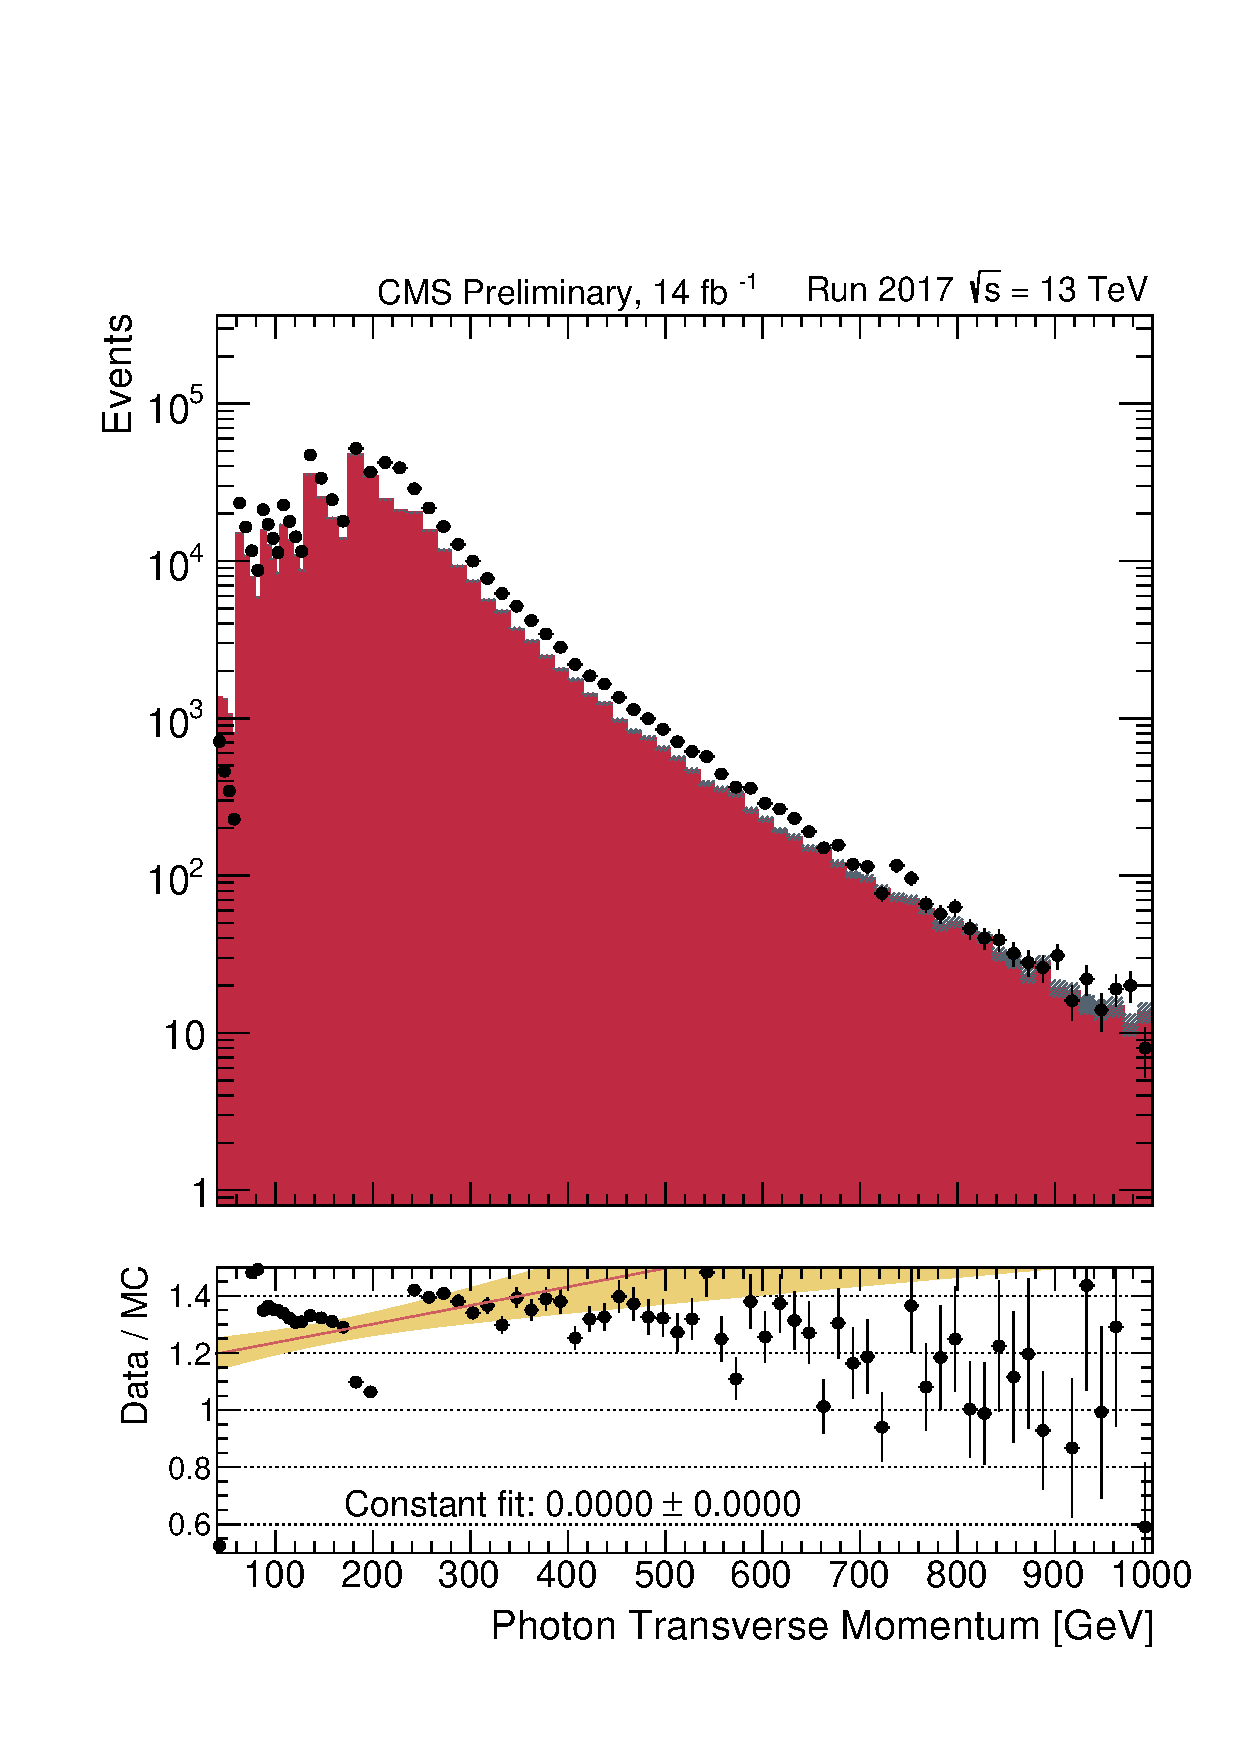
\includegraphics[width=.45\textwidth]{\PhDthesisdir/contents/chapter-JERC/JES/my_plots/distributions/2017UL/with_header/ptPhoton_log.tex}}
\hfill
\subcaptionbox{Énergie transverse manquante.\label{subfig-distrib_Gjets_17UL_MET}}[.45\textwidth]
{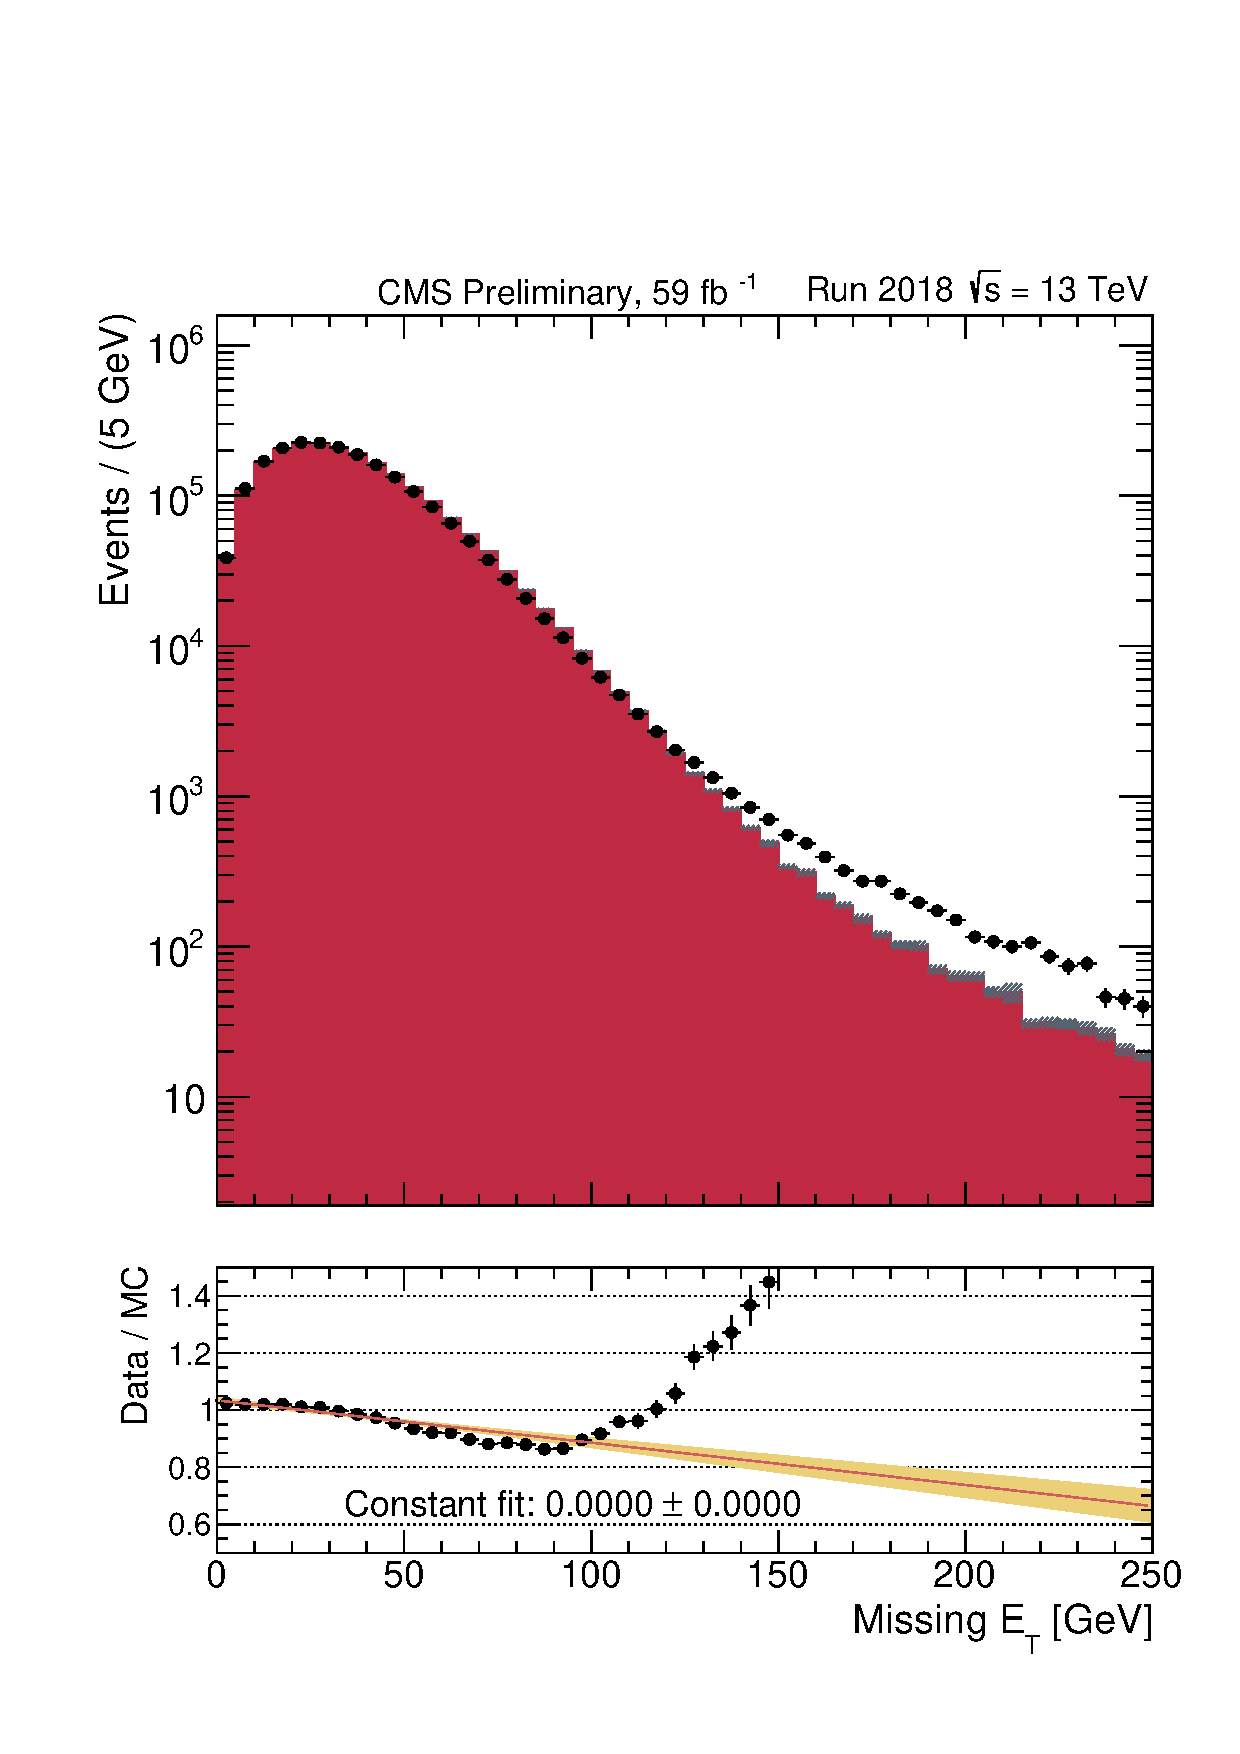
\includegraphics[width=.45\textwidth]{\PhDthesisdir/contents/chapter-JERC/JES/my_plots/distributions/2017UL/with_header/MET_log.tex}}

\vspace{\baselineskip}

\subcaptionbox{Impulsion transverse du premier jet.\label{subfig-distrib_Gjets_17UL_ptFirstJet}}[.45\textwidth]
{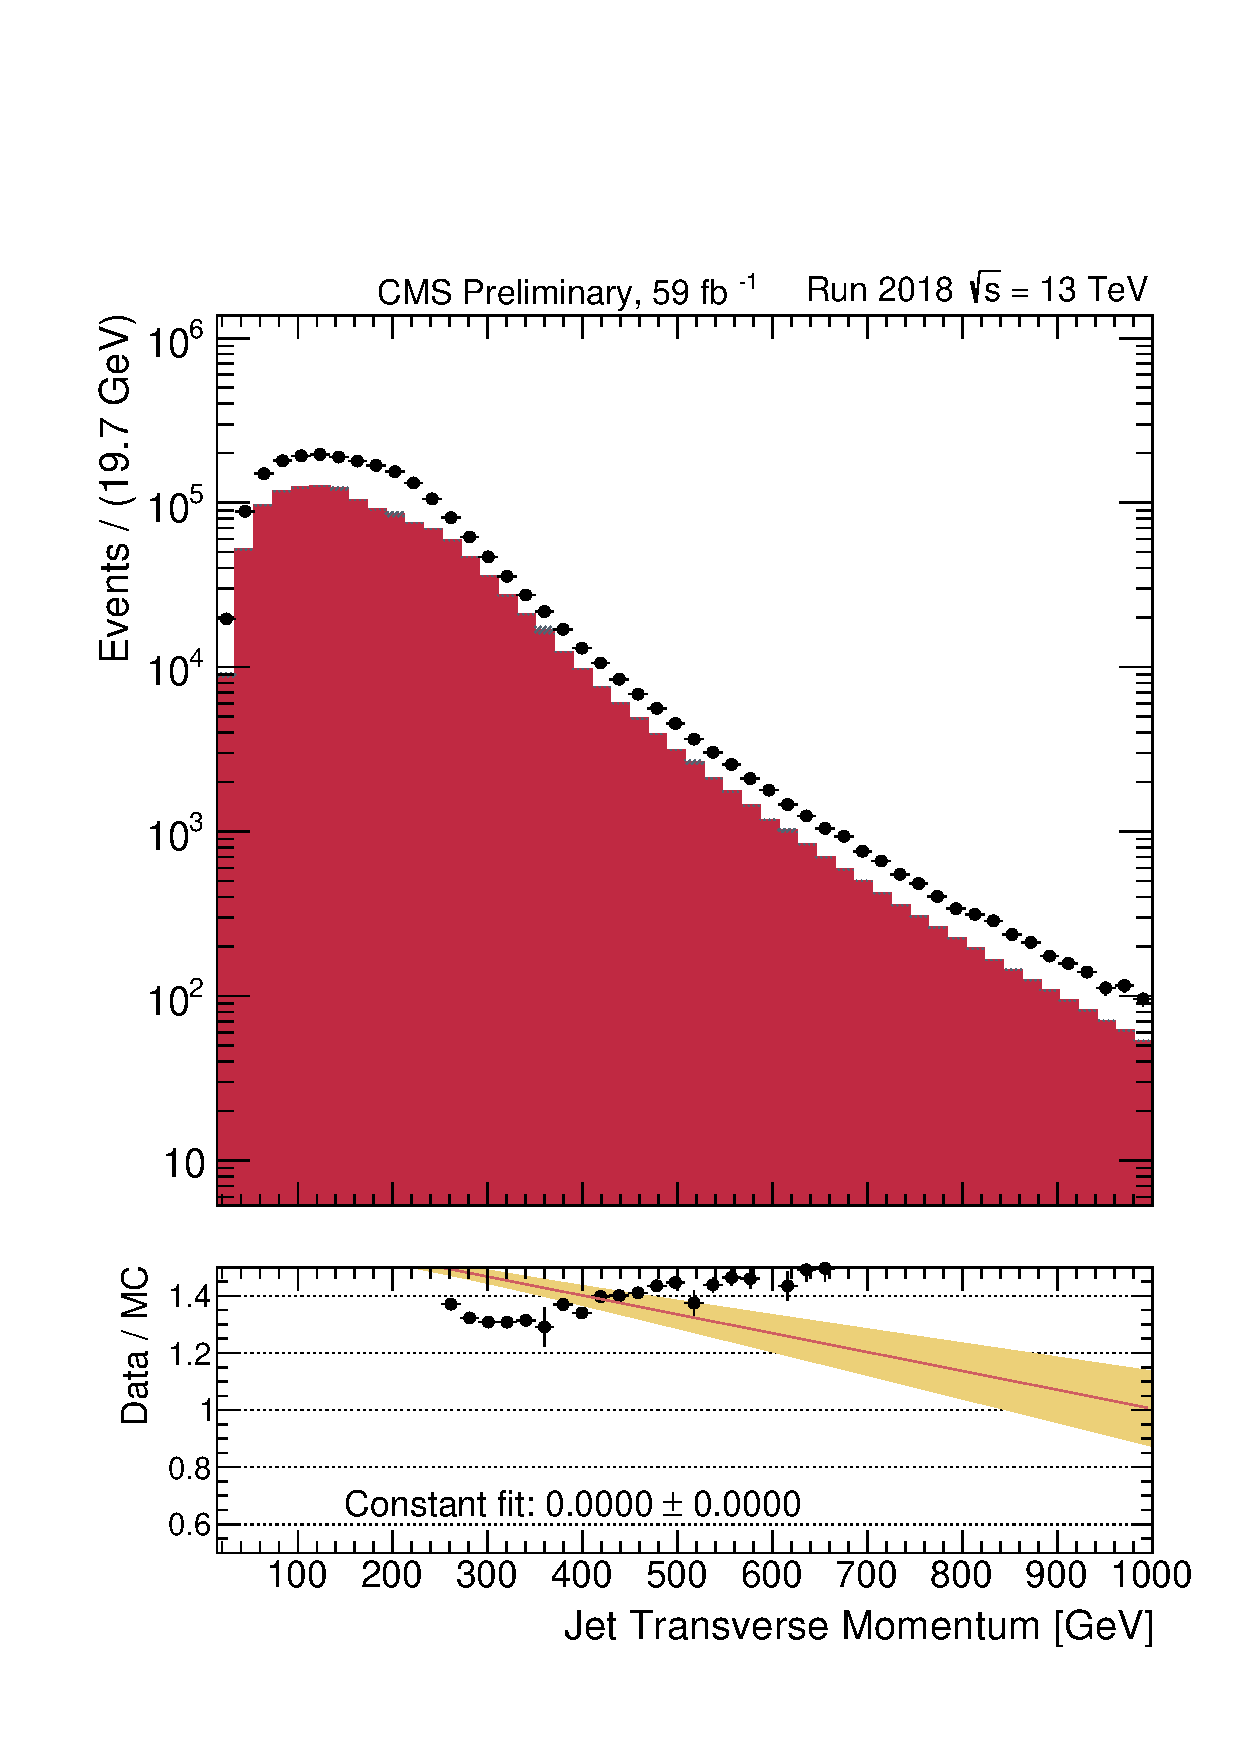
\includegraphics[width=.45\textwidth]{\PhDthesisdir/contents/chapter-JERC/JES/my_plots/distributions/2017UL/with_header/ptFirstJet_log.tex}}
\hfill
\subcaptionbox{Impulsion transverse du second jet.\label{subfig-distrib_Gjets_17UL_ptSecondJet}}[.45\textwidth]
{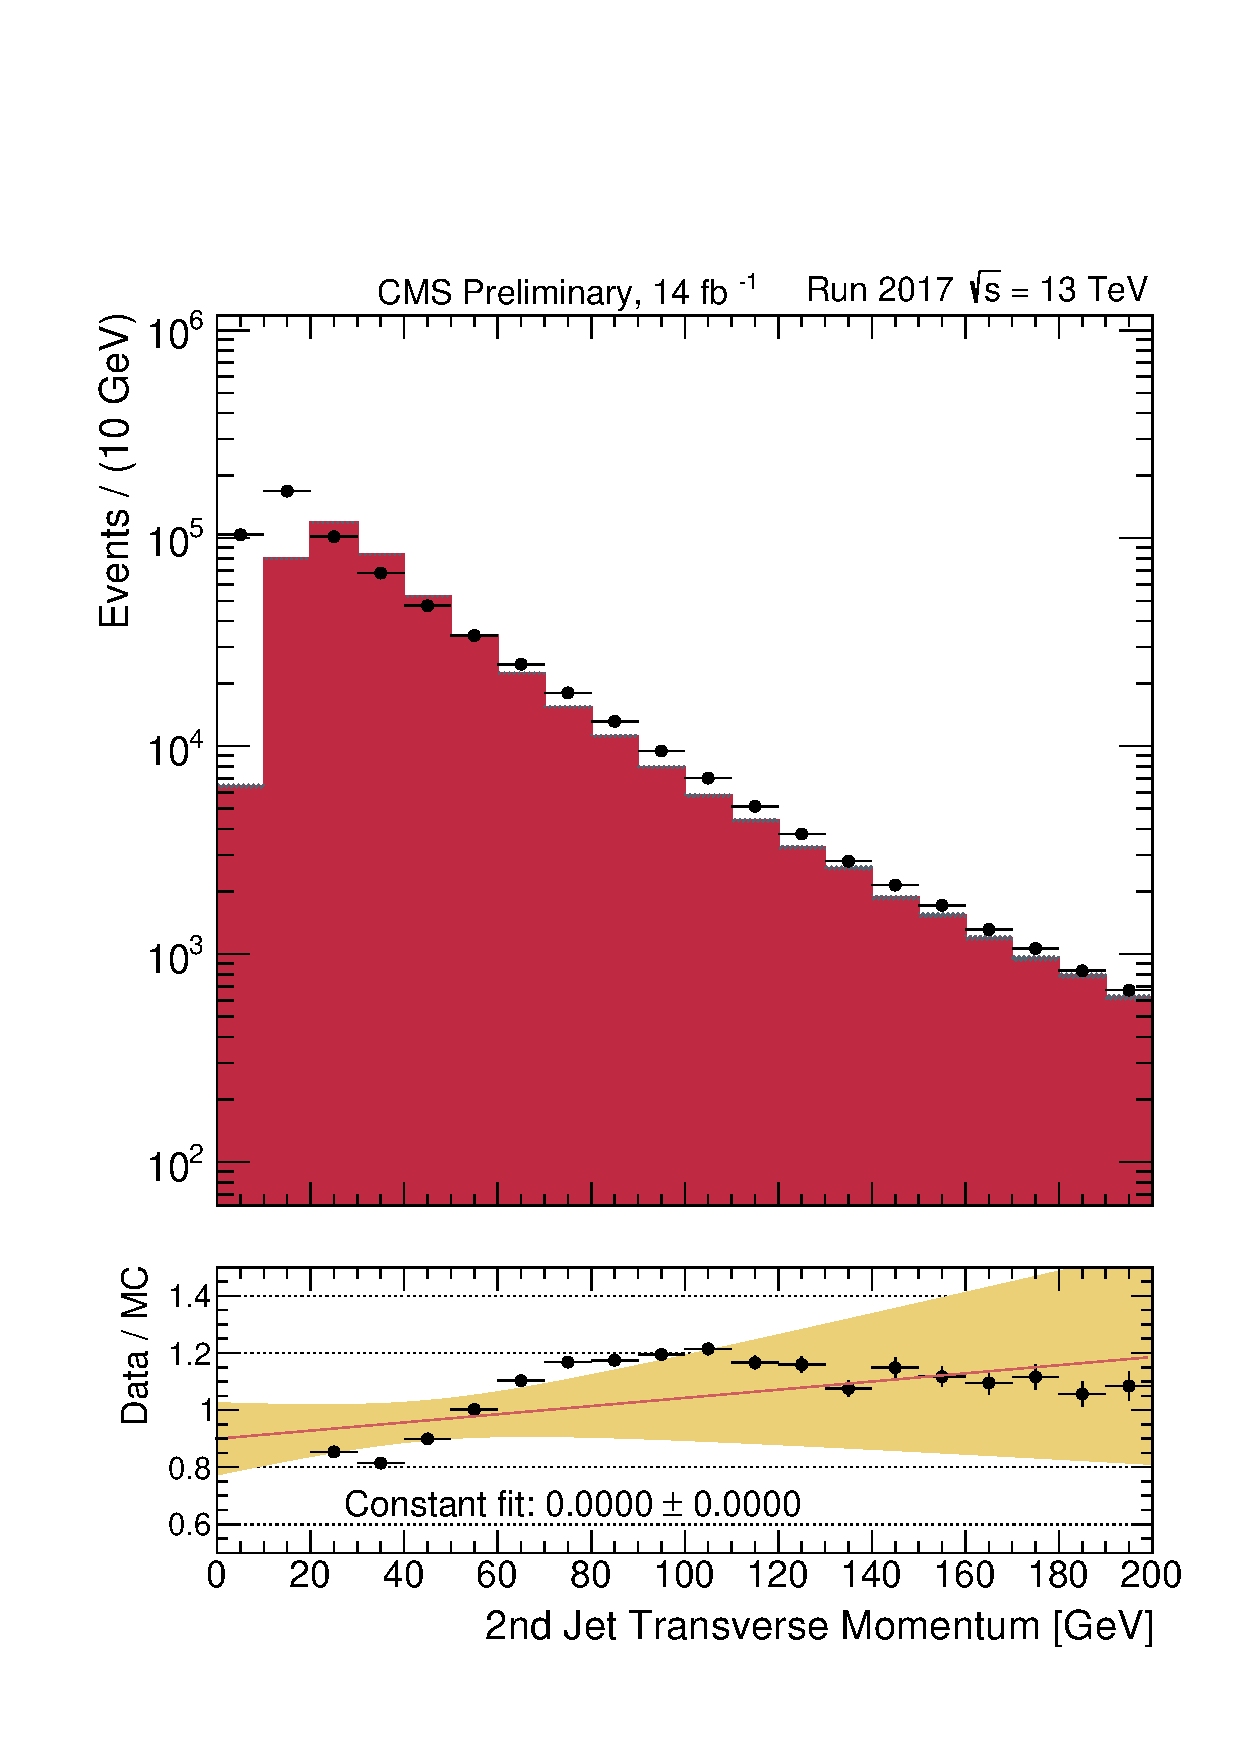
\includegraphics[width=.45\textwidth]{\PhDthesisdir/contents/chapter-JERC/JES/my_plots/distributions/2017UL/with_header/ptSecondJet_log.tex}}

\caption[Observables d'événements \Gjets\ en 2017.]{Distributions d'observables dans les données réelles (points noirs) et simulées (histogramme en rouge) pour l'année 2017-UL.}
\label{fig-distribs_Gjets_17UL}
\end{figure}
\paragraph{Intervalles de $\alpha$}
Comme expliqué dans la section~\ref{chapter-JERC-section-pheno-GJets-subsec-alpha_definition}, l'analyse des événements \Gjets\ est réalisée pour différents intervalles de $\alpha$ afin de pouvoir réaliser par la suite une extrapolation à $\alpha=0$, correspondant au cas idéal d'événements \Gjet.
Les intervalles utilisés sont présentés dans le tableau~\ref{tab-alpha_intervalles}.
Il s'agit d'intervalles inclusifs, \ie\ que chaque intervalle contient l'intervalle précédent.
L'évolution des réponses moyennes en fonction de $\alpha$ y étant linéaire, ce choix rend possible une extrapolation simple vers $\alpha=0$ par la suite.
\begin{table}[h]
\centering
\begin{tabular}{ccccc}
\toprule
$[\num{0}, \num{0.10}[$ & $[\num{0}, \num{0.15}[$ & $[\num{0}, \num{0.20}[$ & $[\num{0}, \num{0.25}[$ & $[\num{0}, \num{0.30}[$ \\
\bottomrule
\end{tabular}
\caption{Intervalles de $\alpha$ utilisés pour la JES.}
\label{tab-alpha_intervalles}
\end{table}
\paragraph{Obtention des corrections pour $(\alpha^\text{max}, \pT^{\photon}, \eta^\text{jet})$ donnés}
Pour chaque domaine
de $\alpha$ défini dans le tableau~\ref{tab-alpha_intervalles},
de $\pT^{\photon}$ défini dans le tableau~\ref{tab-pT_photon_intervalles} et
de $\eta^\text{jet}$ défini dans les tableaux~\ref{tab-eta_jet_intervalles_large} et~\ref{tab-eta_jet_intervalles_fin},
les distributions des réponses balancée et MPF des données réelles et simulées sont déterminées.
Certaines de ces distributions sont représentées sur la figure~\ref{fig-distribs_Gjets_17UL_resp_bal_and_mpf}.

\todo{98.5 pct RMS, mean}

\par \todo{TODO}: only eta photon < 1.3 for the moment (barrel) (already said ? check non ambiguous with eta jet) + future with all photons


\begin{figure}[h]
\centering
\subcaptionbox{Réponse balancée pour $\pT^{\photon}\in[175, 230[$ \SI{}{\GeV}.\label{subfig-distrib_Gjets_17UL_resp_balancing_eta0013_ptPhot_175_230}}[.45\textwidth]
{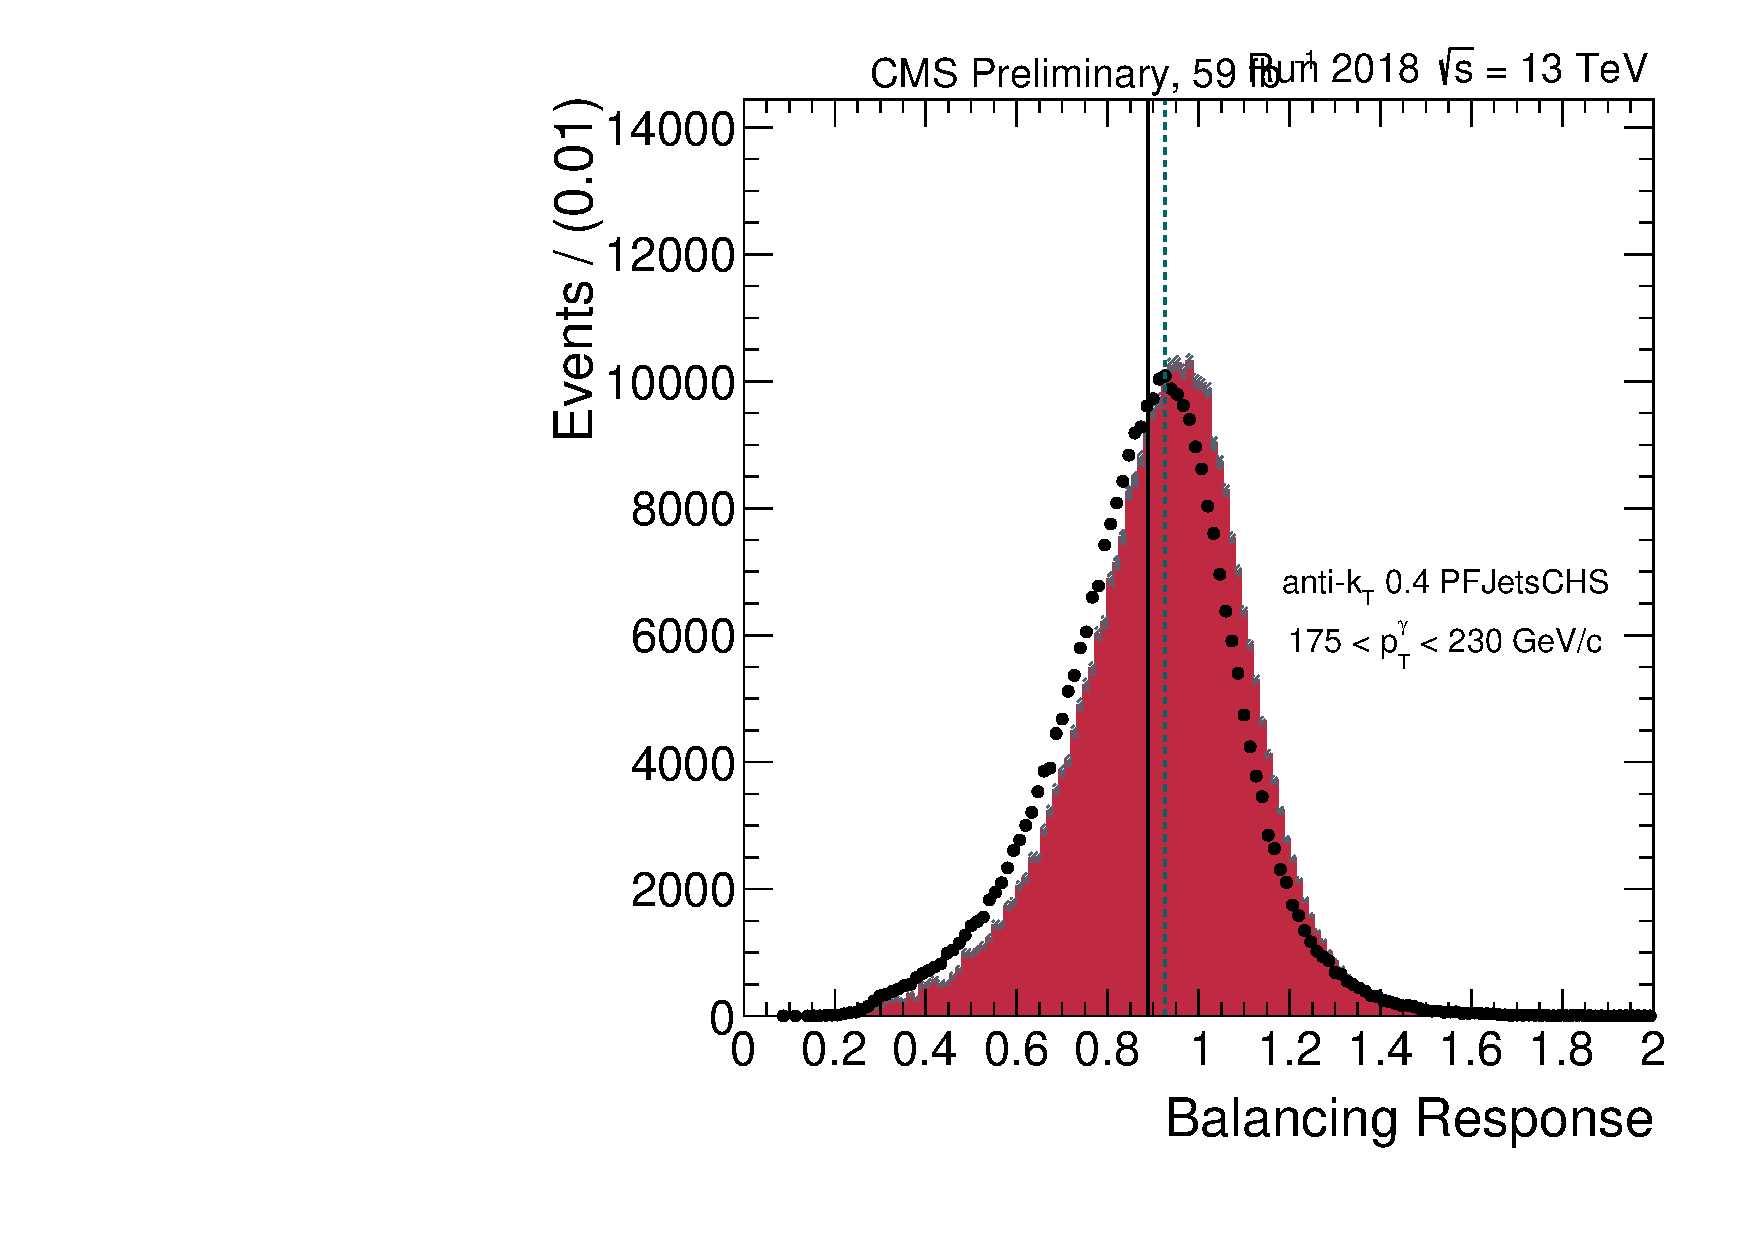
\includegraphics[width=.45\textwidth]{\PhDthesisdir/contents/chapter-JERC/JES/my_plots/distributions/2017UL/with_header/resp_balancing_eta0013_ptPhot_175_230.tex}}
\hfill
\subcaptionbox{Réponse balancée pour $\pT^{\photon}\in[300, 400[$ \SI{}{\GeV}.\label{subfig-distrib_Gjets_17UL_resp_balancing_eta0013_ptPhot_300_400}}[.45\textwidth]
{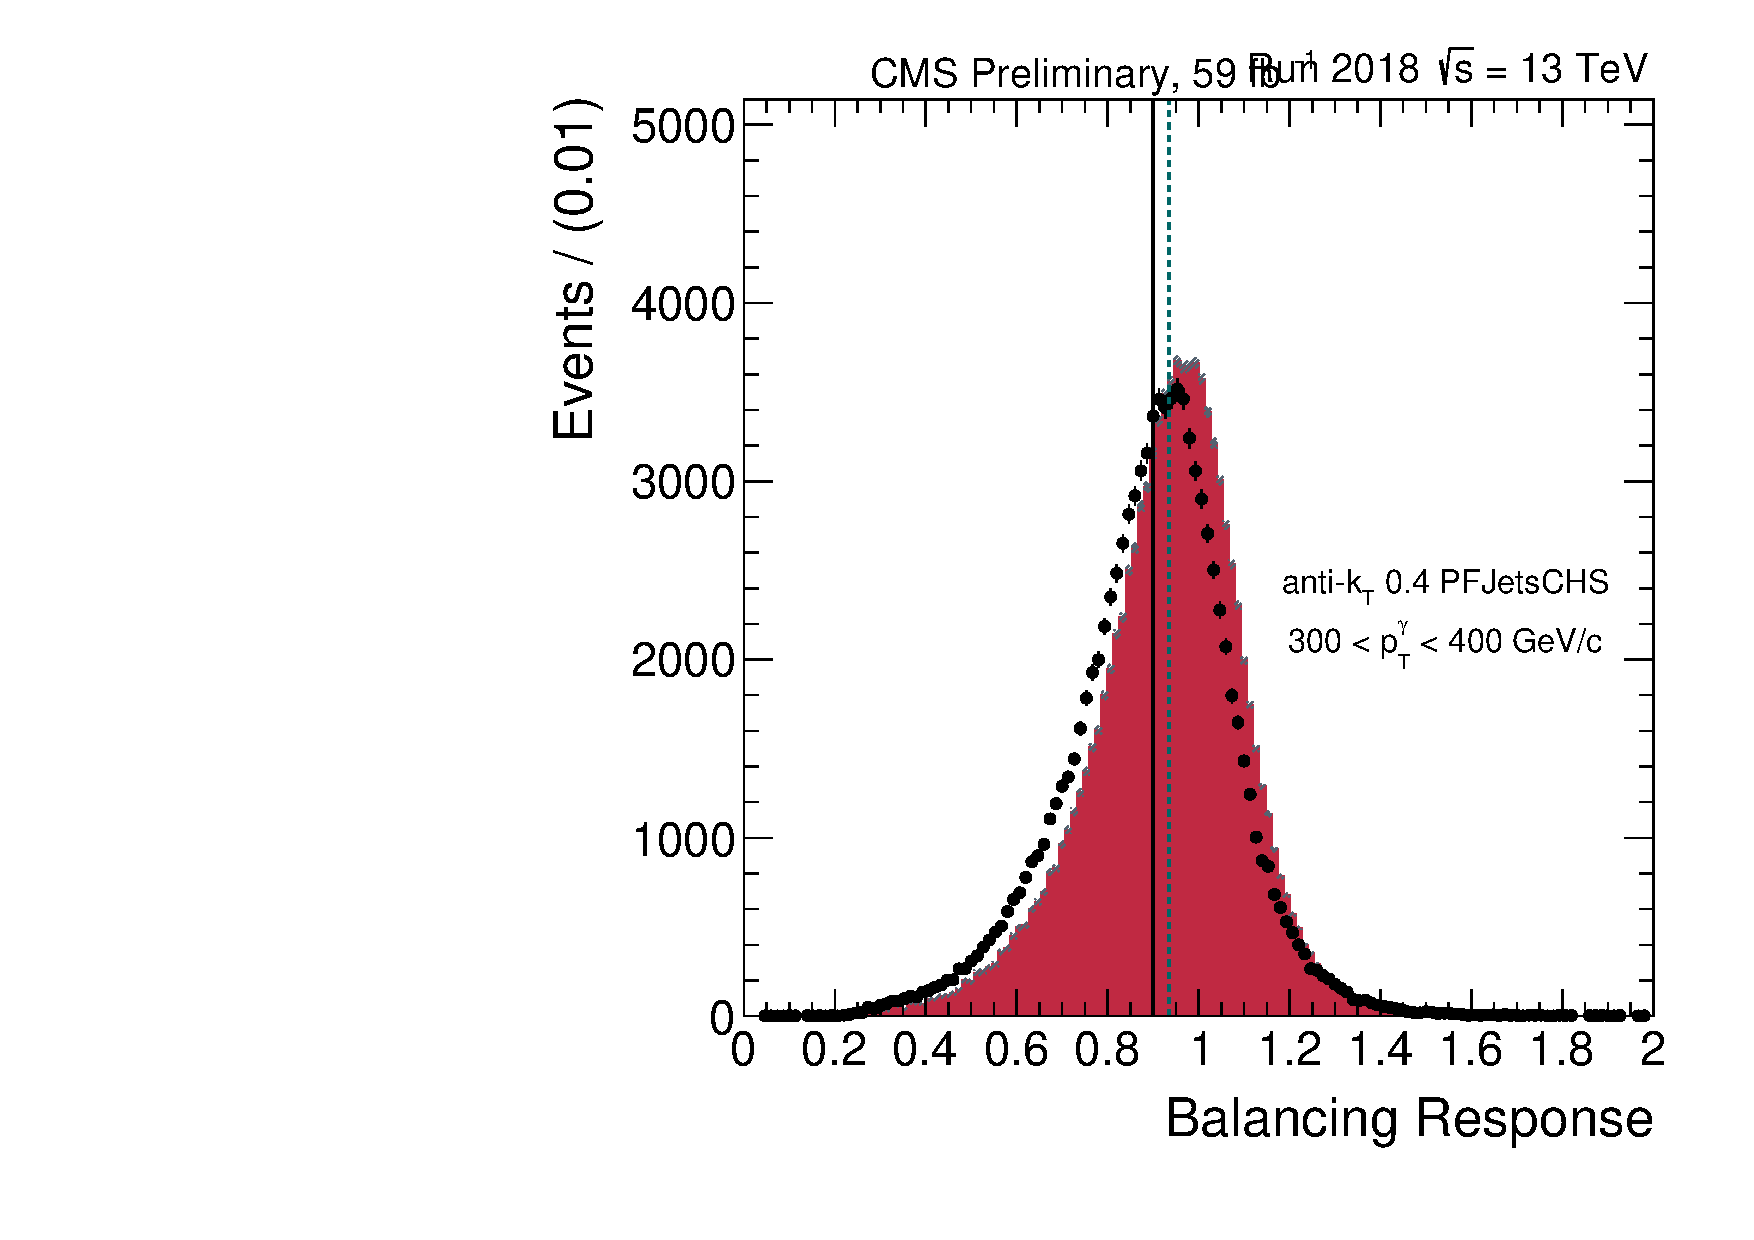
\includegraphics[width=.45\textwidth]{\PhDthesisdir/contents/chapter-JERC/JES/my_plots/distributions/2017UL/with_header/resp_balancing_eta0013_ptPhot_300_400.tex}}

\vfill

\subcaptionbox{Réponse MPF pour $\pT^{\photon}\in[175, 230[$ \SI{}{\GeV}.\label{subfig-distrib_Gjets_17UL_resp_mpf_eta0013_ptPhot_175_230}}[.45\textwidth]
{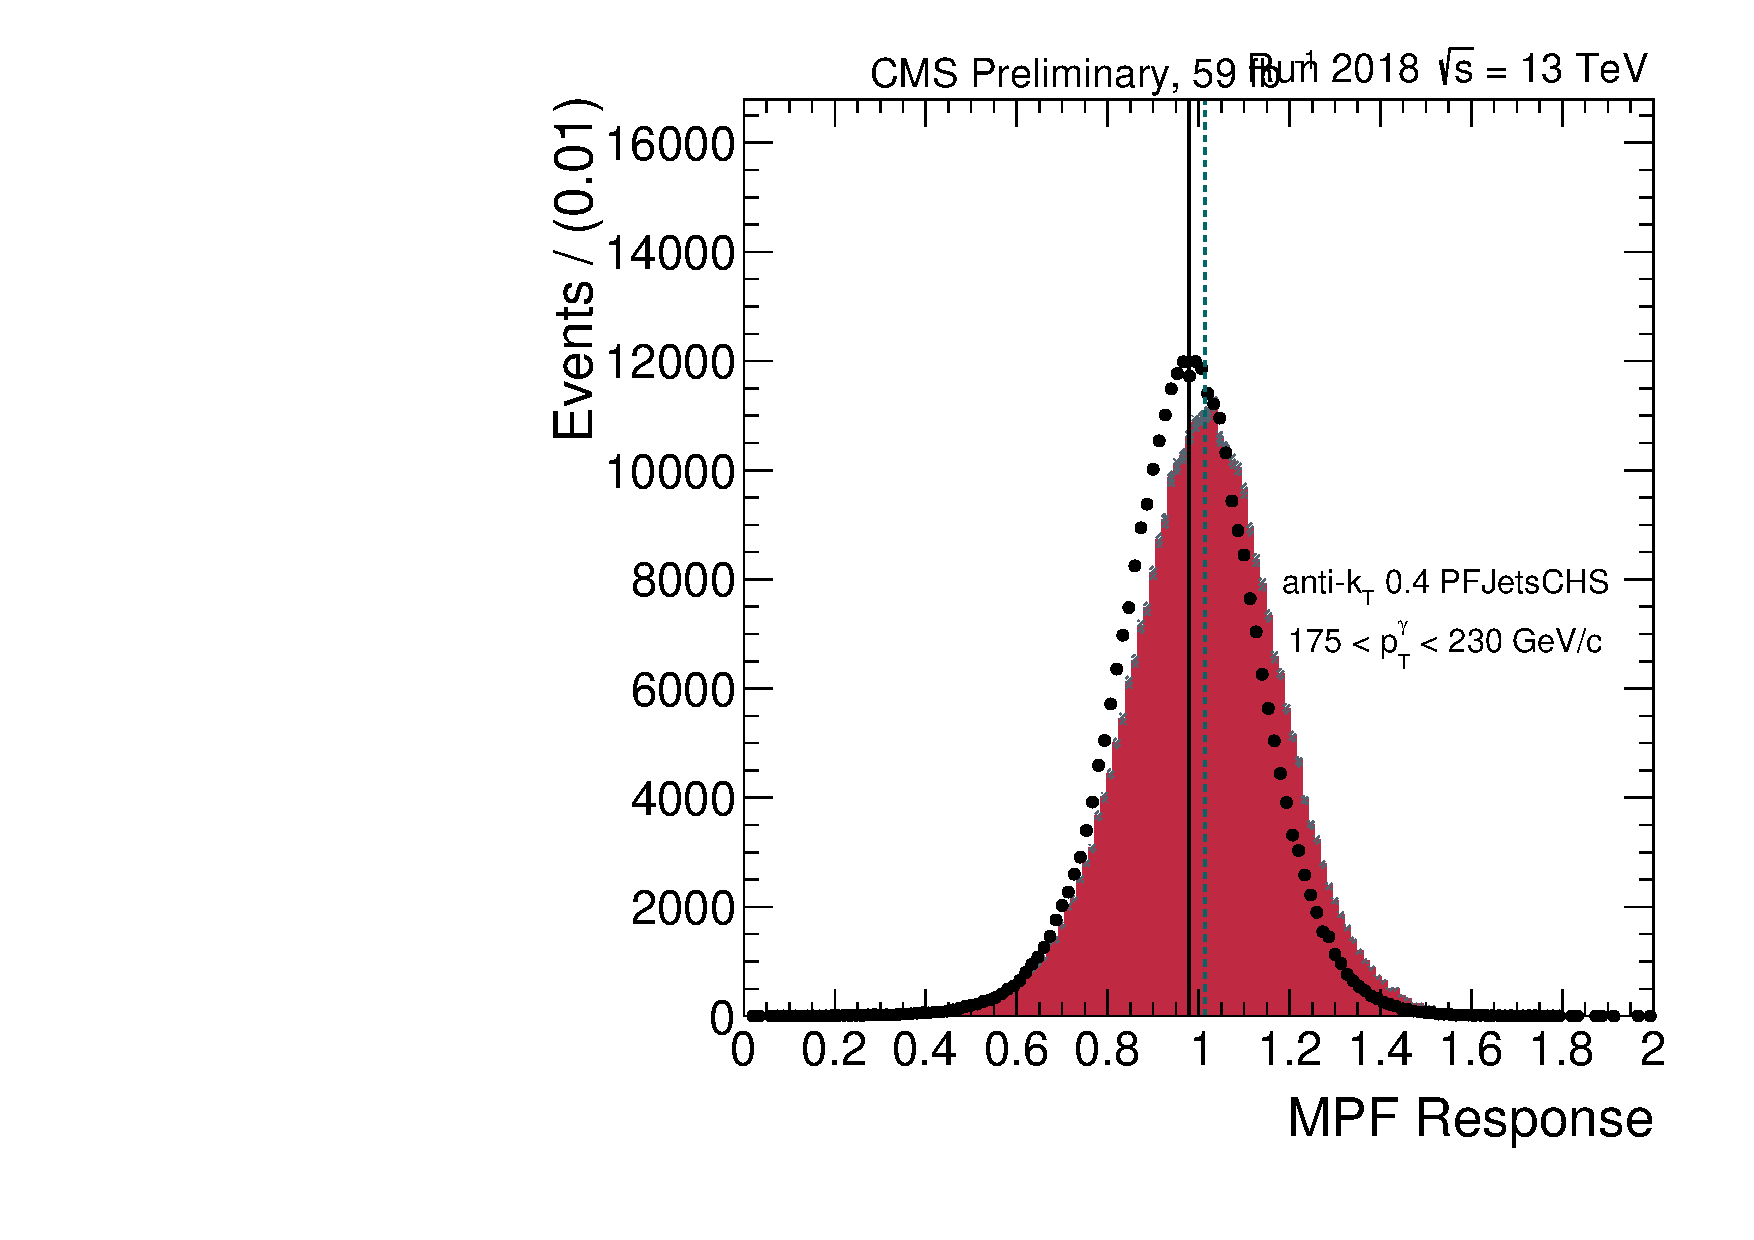
\includegraphics[width=.45\textwidth]{\PhDthesisdir/contents/chapter-JERC/JES/my_plots/distributions/2017UL/with_header/resp_mpf_eta0013_ptPhot_175_230.tex}}
\hfill
\subcaptionbox{Réponse MPF pour $\pT^{\photon}\in[300, 400[$ \SI{}{\GeV}.\label{subfig-distrib_Gjets_17UL_resp_mpf_eta0013_ptPhot_300_400}}[.45\textwidth]
{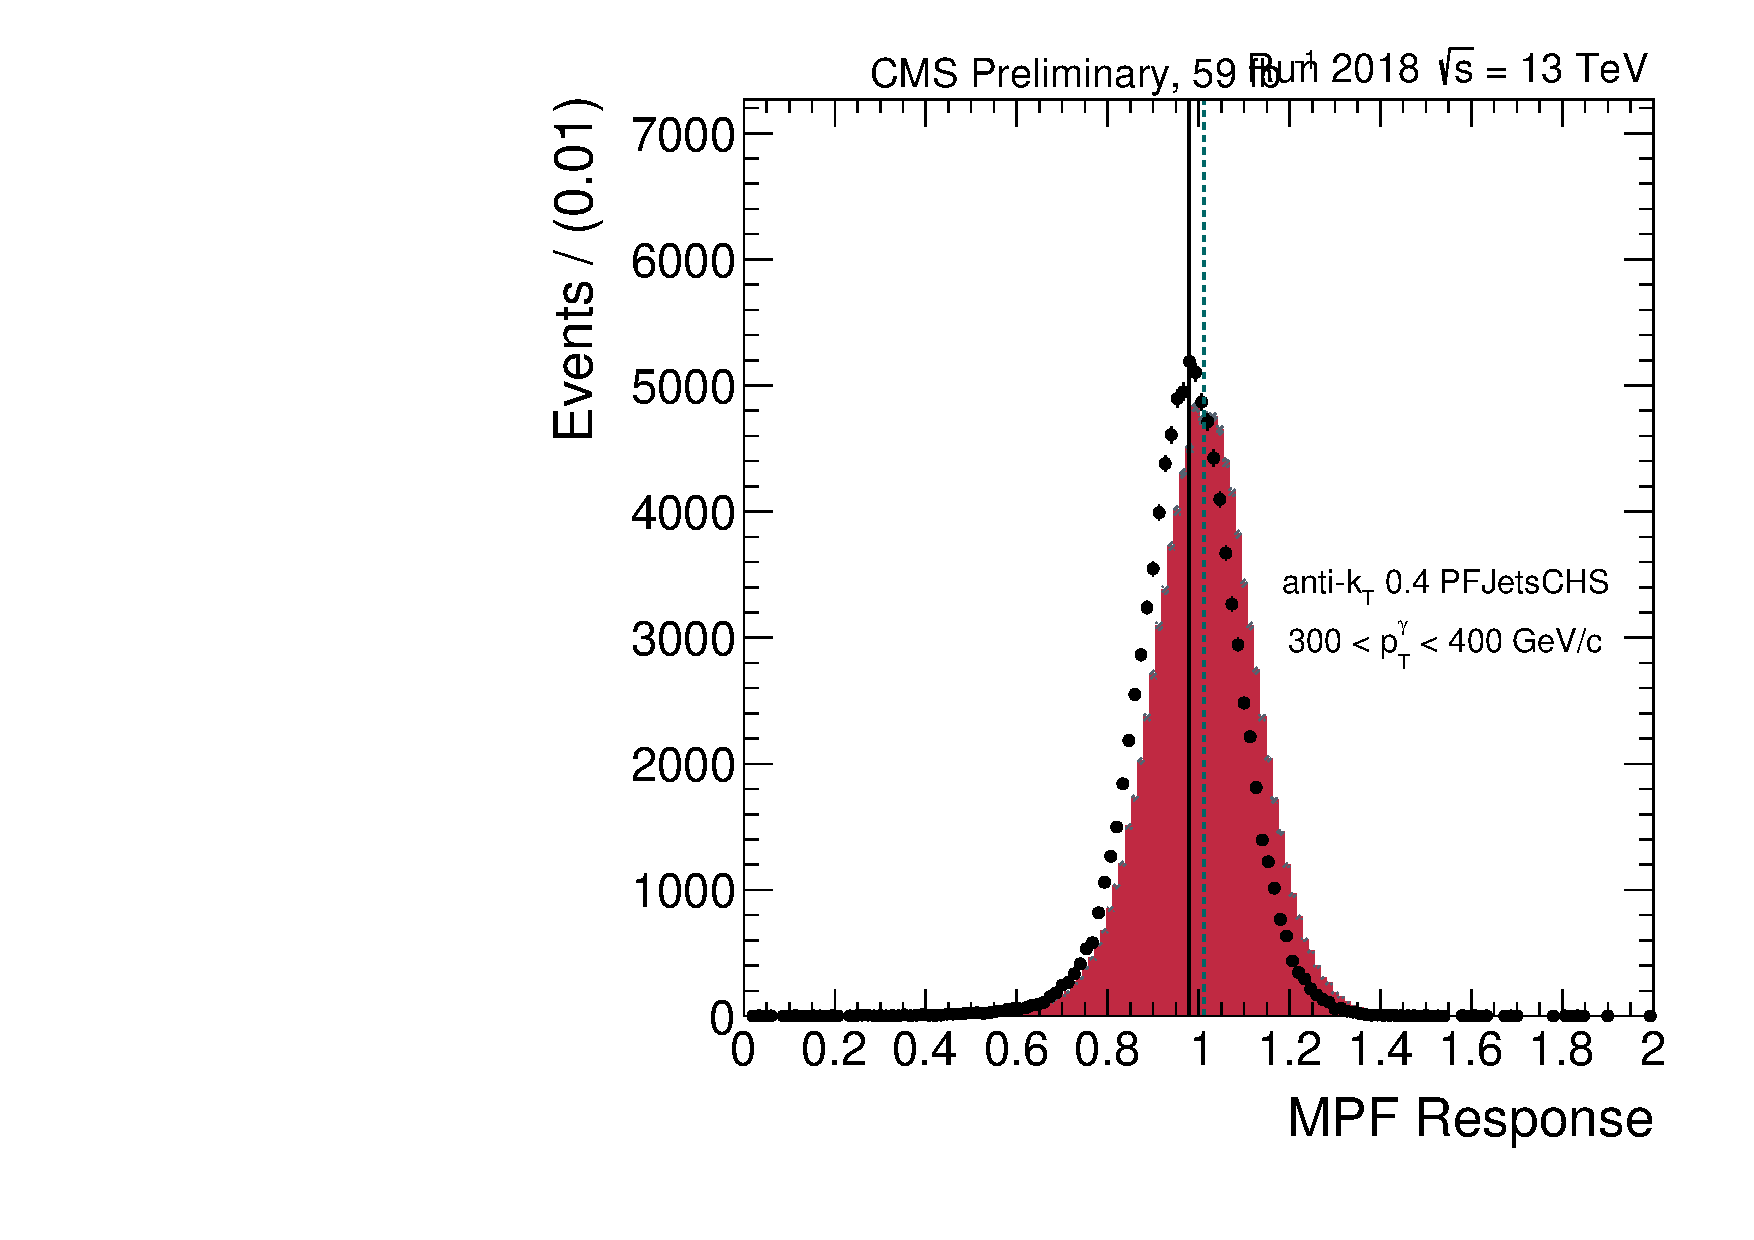
\includegraphics[width=.45\textwidth]{\PhDthesisdir/contents/chapter-JERC/JES/my_plots/distributions/2017UL/with_header/resp_mpf_eta0013_ptPhot_300_400.tex}}

\caption[Réponses balancée et MPF en 2017-UL.]{Réponses balancée et MPF dans les données réelles (points noirs) et simulées (histogramme en rouge) pour $\alpha<\num{0.3}$, $\abs{\eta^\text{jet}}<\num{1.3}$ et deux intervalles de $\pT^{\photon}$ en 2017-UL.}
\label{fig-distribs_Gjets_17UL_resp_bal_and_mpf}
\end{figure}


\paragraph{Extrapolation vers $\alpha=0$}
\todo{rappel de la figure dans section précédente}


%\subsection{Incertitudes}\label{chapter-JERC-section-JES-subsec-uncertainties}

\subsection{Résultats}\label{chapter-JERC-section-JES-subsec-results}
\todo{avant et après extrap.}